\documentclass{beamer}
\usepackage{graphicx}
\usepackage{amsmath}
\usepackage{tikz,pgfplots}
\pgfplotsset{compat=1.17}
\usepackage{caption}
\usepackage{subcaption}
\usetheme{Madrid}

\title{Spacecraft Attitude Control using Reaction Wheels}
\author{Alan Siby \and Allison Byrnes}
\date{\today}

\begin{document}

% --- Title Slide ---
\begin{frame}
  \titlepage
\end{frame}

% --- Outline ---
\begin{frame}{Outline}
  \tableofcontents
\end{frame}

\section{Introduction}
\begin{frame}{What is Spacecraft Attitude Control?}
\begin{itemize}
  \item \textbf{Attitude} refers to the orientation of a spacecraft in space—its angular position relative to a reference frame (e.g., Earth, stars, or orbit path).
  
  \item \textbf{Attitude control} is the process of actively adjusting or maintaining this orientation using actuators such as:
  \begin{itemize}
    \item Reaction wheels
    \item Control moment gyroscopes
    \item Magnetorquers
    \item Thrusters
  \end{itemize}
\end{itemize}
\end{frame}

% --- Motivation ---
\begin{frame}{Why Is it Important?}
\begin{itemize}
  \item Precise orientation is vital for:
  \begin{itemize}
    \item Imaging missions
    \item Communications
    \item Orbital maneuvers
  \end{itemize}
  \item Enable high-precision line-of-sight stability without fuel
\end{itemize}
\end{frame}

% --- Objectives ---
\begin{frame}{Project Objectives}
\begin{itemize}
  \item Simulate spacecraft attitude control in Python
  \item Implement PD controller with saturation and torque limits
  \item Design for performance:
  \begin{itemize}
    \item Settling time $< 5$ s
    \item Overshoot $< 2^\circ$
  \end{itemize}
  \item Find the most optimal gains
  \item Compare performance across spacecraft sizes
\end{itemize}
\end{frame}


\section{Dynamics}
\begin{frame}{Governing Dynamics}
\begin{block}{Reaction Wheel Torque}
    \begin{center}
        $\tau = I_{rw} \dot{\omega}$
    \end{center}
\end{block}
\begin{block}{Control Law (PD)}
    \begin{center}
        $\tau = -k_1 e - k_2 \dot{e}$
    \end{center}
\end{block}
\begin{block}{Closed Loop}
    \begin{center}
        $I_{sc} \ddot{\theta} + k_2 \dot{\theta} + k_1 \theta = 0$
    \end{center}
\end{block}
\end{frame}


\begin{frame}{Dynamics - State Space Equations}
\begin{block}{State-Space Equation}
\begin{align}
    \dot{x}(t) &= Ax(t) + Bu(t) \\
    y(t) &= Cx(t) + Du(t)
\end{align}
\end{block}
\begin{block}{States}
    \begin{equation}
        \mathbf{x}(t) = \begin{bmatrix} \theta(t) \\ \omega_{sc}(t) \end{bmatrix}
    \end{equation}
\end{block}
\begin{block}{Command Torque}
    \begin{equation}
        \tau_{cmd}(t) = -k_1 \theta(t) - k_2 \omega_{sc}(t)
    \end{equation}
\end{block}
\end{frame}

\begin{frame}{Dynamics - State Space Equations}
\begin{block}{Kinematic Equation}
    \begin{equation}
        \dot{\theta}(t) = \omega_{sc}(t)
    \end{equation} 
\end{block}

\begin{block}{Dynamic Equation}
    \begin{equation}
        \dot{\omega}_{sc}(t) = -\frac{k_1}{I_{sc}} \theta(t) - \frac{k_2}{I_{sc}} \omega_{sc}(t)
    \end{equation}
\end{block}
\end{frame}




\begin{frame}{Characteristic Equation - Setup}
\begin{block}{Characteristic Equation}
    \begin{equation}
        \det(sI - A) = s^2 + \frac{k_2}{I_{sc}}s + \frac{k_1}{I_{sc}} = 0
    \end{equation}   
\end{block}
\end{frame}


\section{Simulation Setup}

% --- Test Cases ---
\begin{frame}{Test Cases}
\begin{columns}
\begin{column}{0.5\textwidth}
\textbf{Large Spacecraft} (3 cases):
\begin{itemize}
  \item Inertia: $1{,}000~\text{kg}\cdot\text{m}^2$
  \item Wheel: $1$--$20~\text{kg}\cdot\text{m}^2$
  \item Max speed: $3{,}000$--$25{,}000$ RPM
  \item Max torque: $2$--$50$ Nm
\end{itemize}
\end{column}
\begin{column}{0.5\textwidth}
\textbf{Small Spacecraft} (3 cases):
\begin{itemize}
  \item Inertia: $10~\text{kg}\cdot\text{m}^2$
  \item Wheel: $0.05$--$0.5~\text{kg}\cdot\text{m}^2$
  \item Max speed: $500$--$30{,}000$ RPM
  \item Max torque: $0.1$--$1$ Nm
\end{itemize}
\end{column}
\end{columns}

\vspace{0.3cm}
\textbf{Test Conditions:}
\begin{itemize}
  \item Manually input values of $k_1 = 4.0$ \& $k_2 = 10.0$
  \item $10^\circ$ step disturbance
  \item Requirements: $T_s < 5$ s, overshoot $< 2^\circ$
  \item Full parameter space sweep
\end{itemize}
\end{frame}

\section{Results}

% --- Small Spacecraft Time Domain ---
\begin{frame}{Large Spacecraft Results - Time Domain \& Analysis}
    \begin{figure}[H]
    \label{Fig. 1}
    \centering
    \begin{subfigure}[b]{0.48\columnwidth}
        \label{Fig. 1.A}
        \centering
        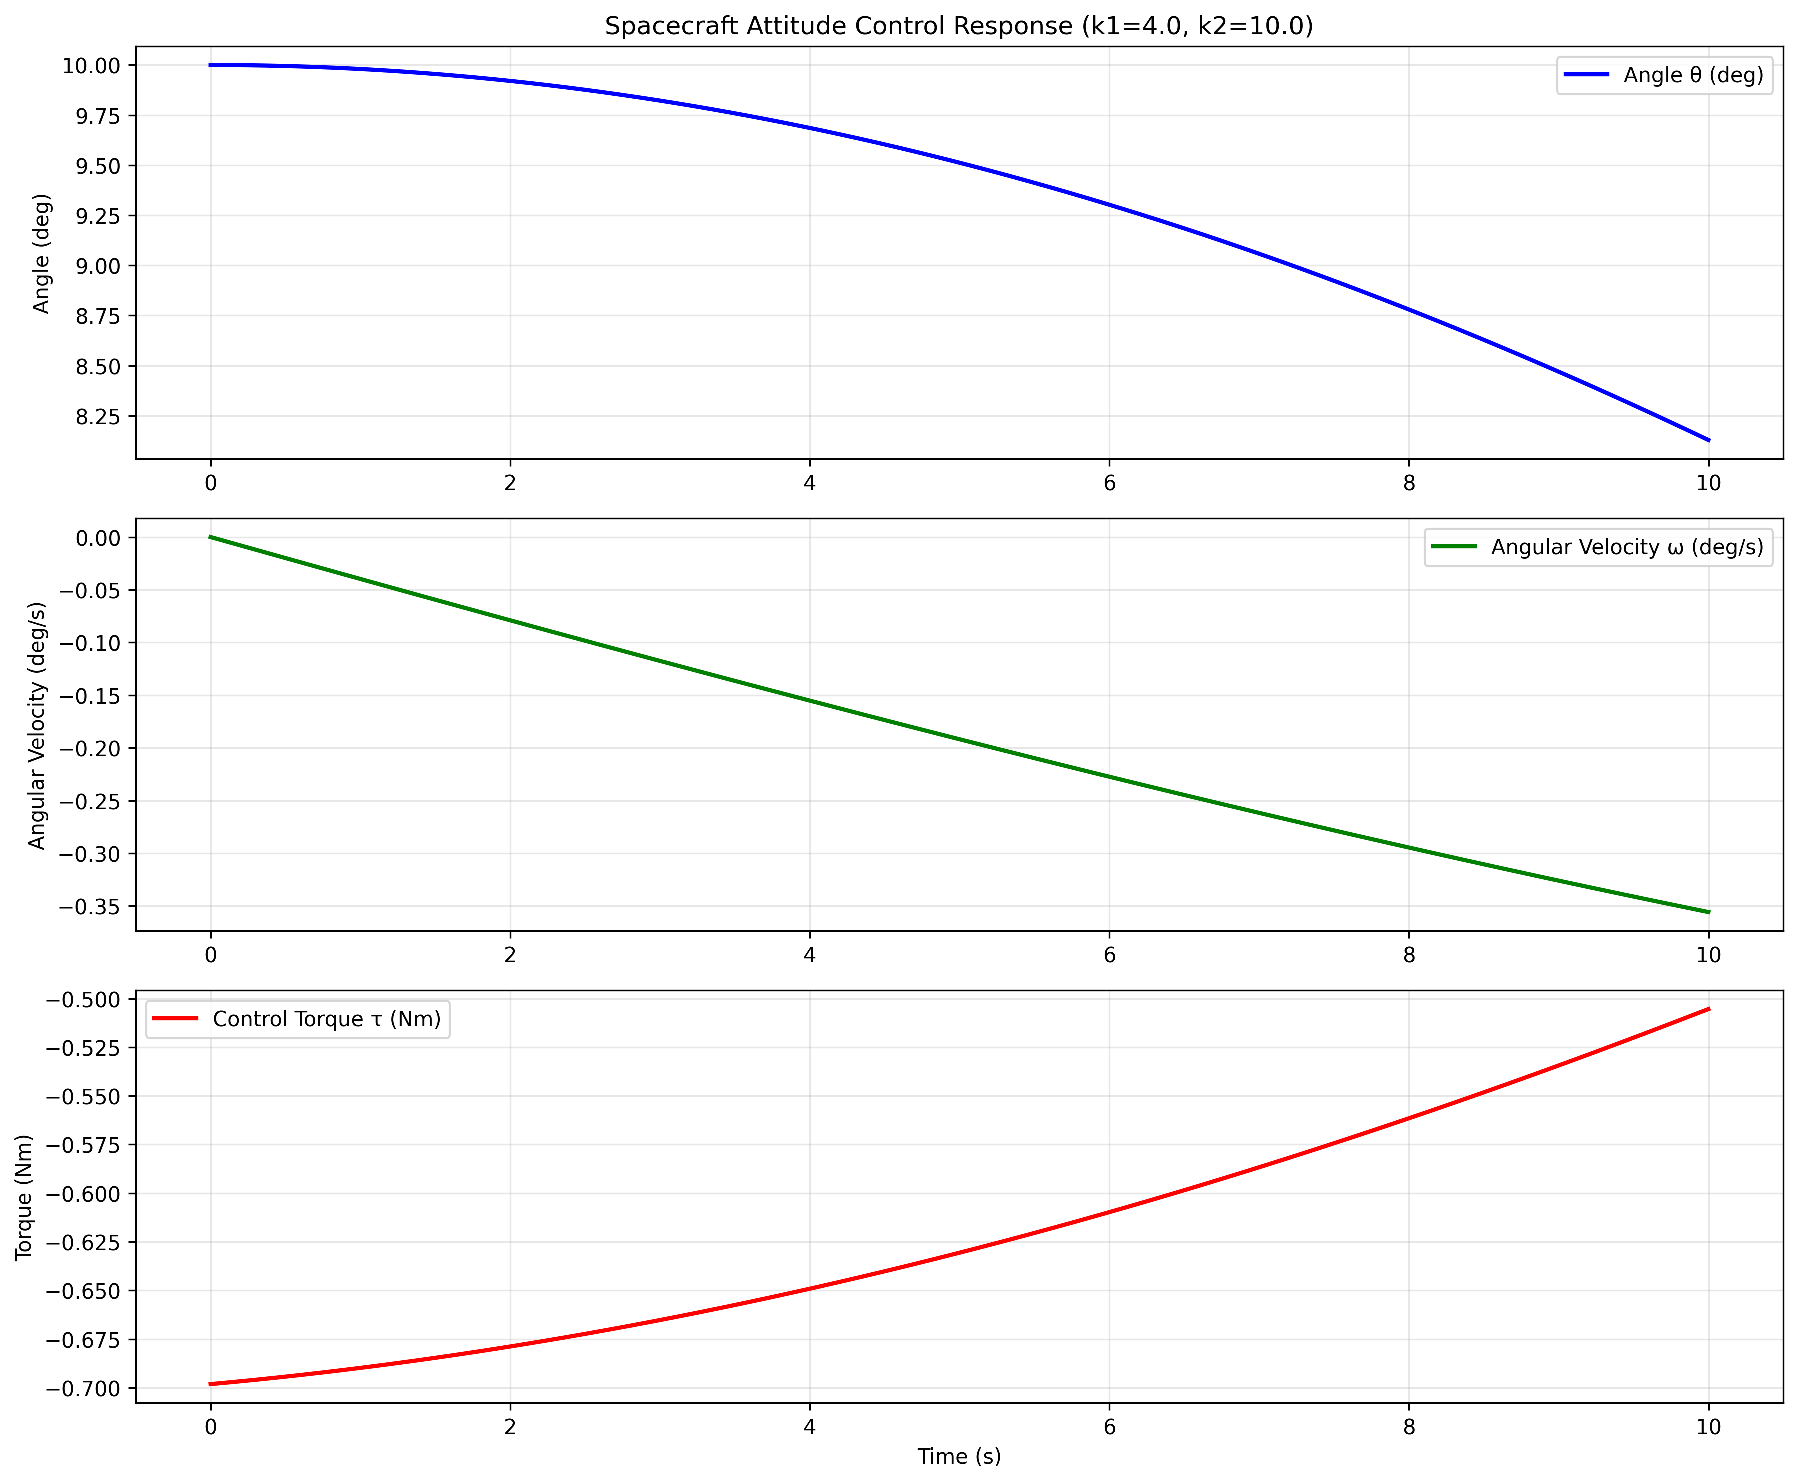
\includegraphics[width=\linewidth]{base_time_domain(1).pdf}
        \caption{Time-domain graphs}
        \label{fig:subfig1}
    \end{subfigure}
    \hfill
    \begin{subfigure}[b]{0.48\columnwidth}
        \label{Fig. 1.B}
        \centering
        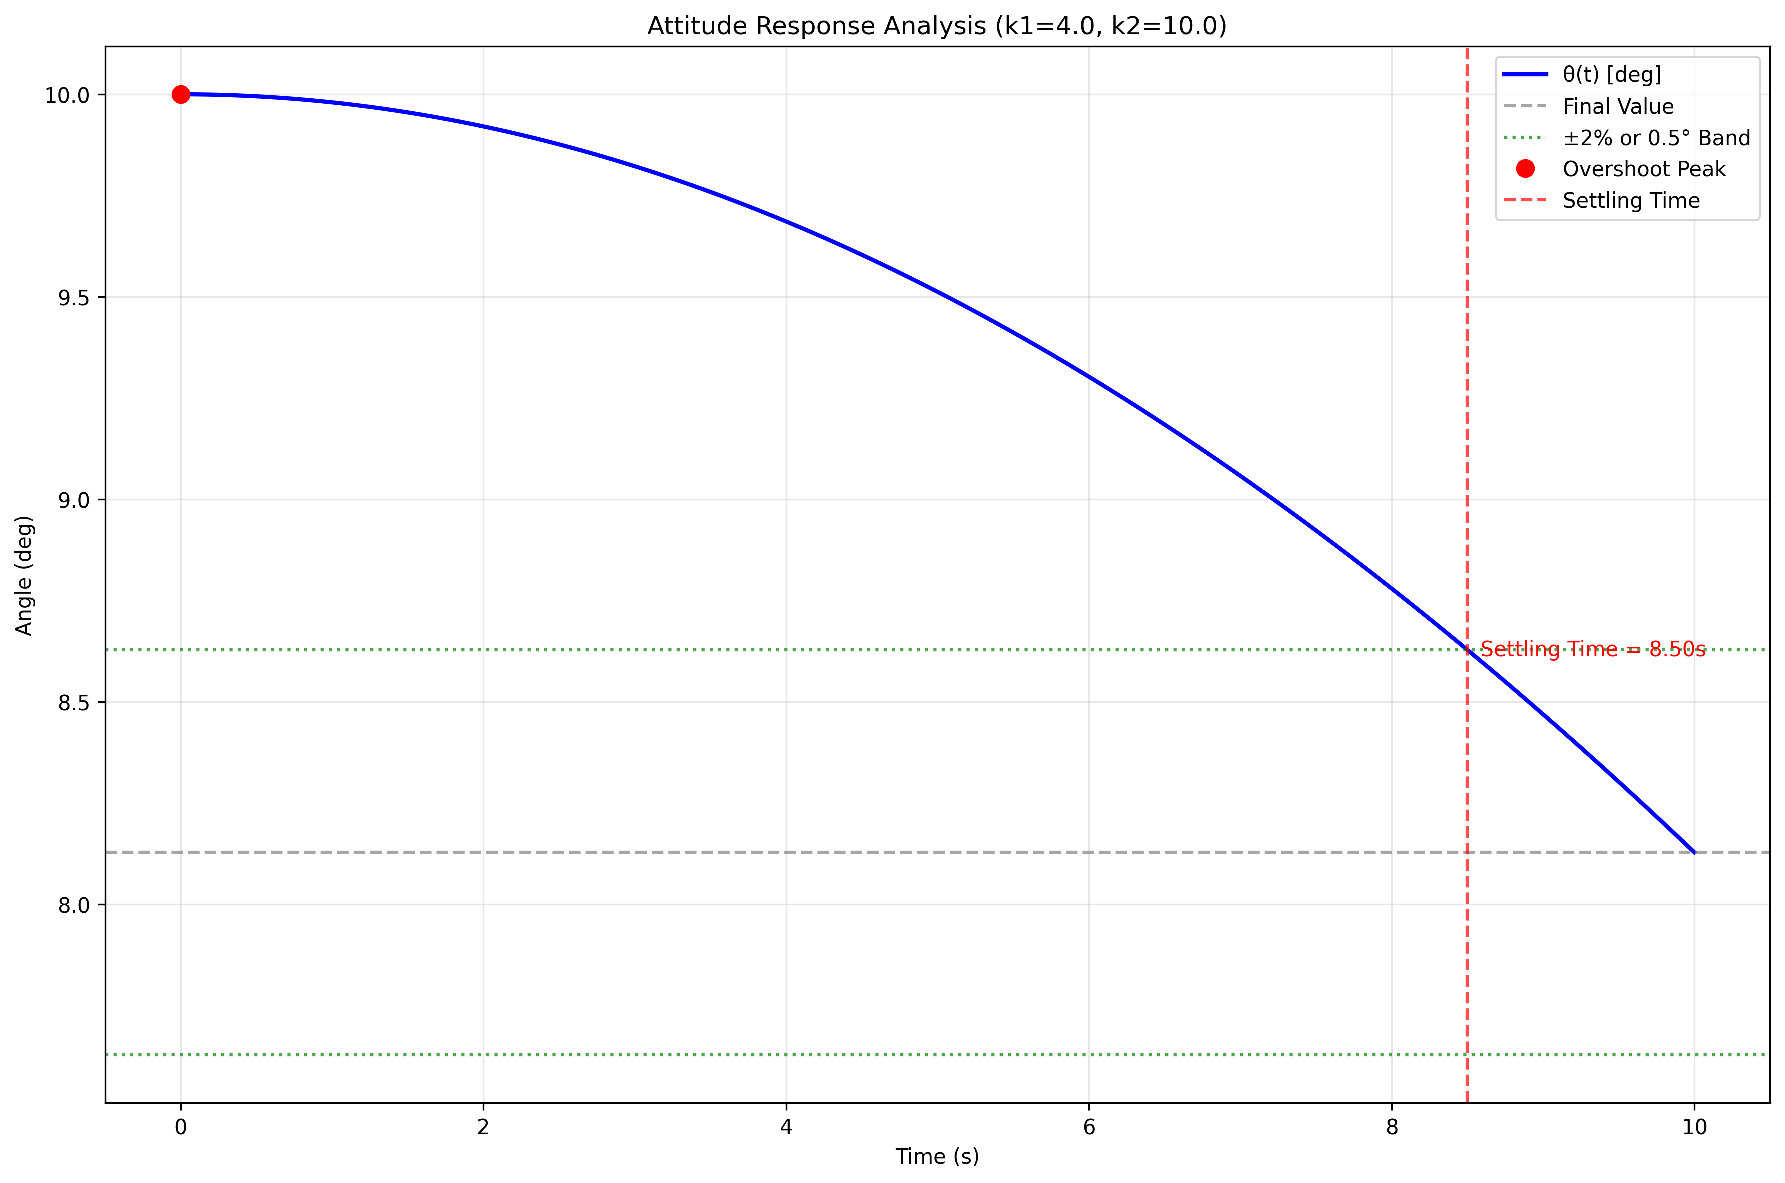
\includegraphics[width=\linewidth]{base_analysis(1).pdf}
        \caption{Response analysis graph}
        \label{fig:subfig2}
    \end{subfigure}
    \caption{Time-domain and Analysis of manually input gains for large spacecraft case 1}
    \label{fig:combined}
\end{figure}
\end{frame}

\begin{frame}{Large Spacecraft Results - Root Locus}
    \begin{figure}[H]
    \label{Fig. 1}
    \centering
    \begin{subfigure}[b]{0.48\columnwidth}
        \label{Fig. 1.A}
        \centering
        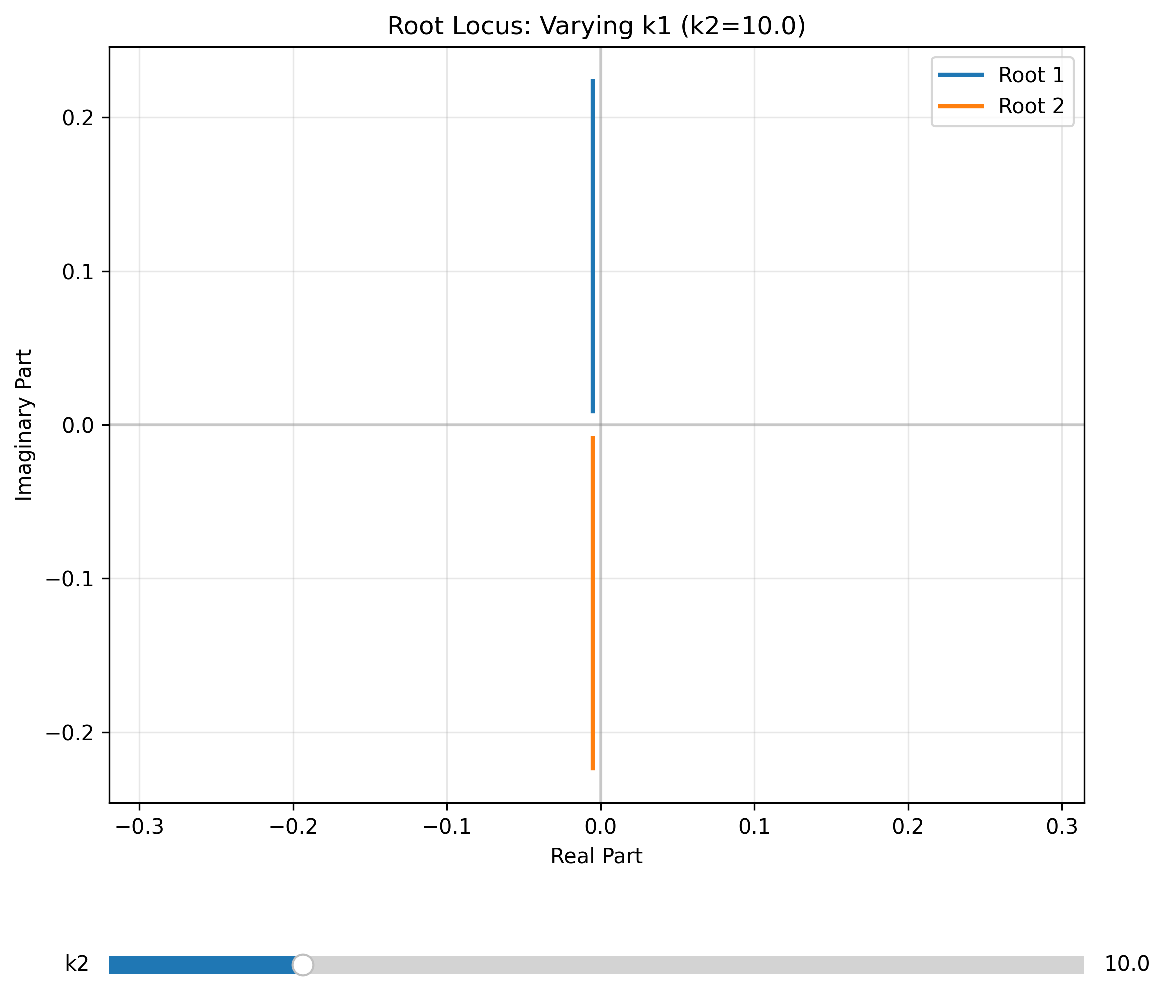
\includegraphics[width=\linewidth]{base_k1__root_locus(1).pdf}
        \caption{Fixed $k_2$}
        \label{fig:subfig1}
    \end{subfigure}
    \hfill
    \begin{subfigure}[b]{0.48\columnwidth}
        \label{Fig. 1.B}
        \centering
        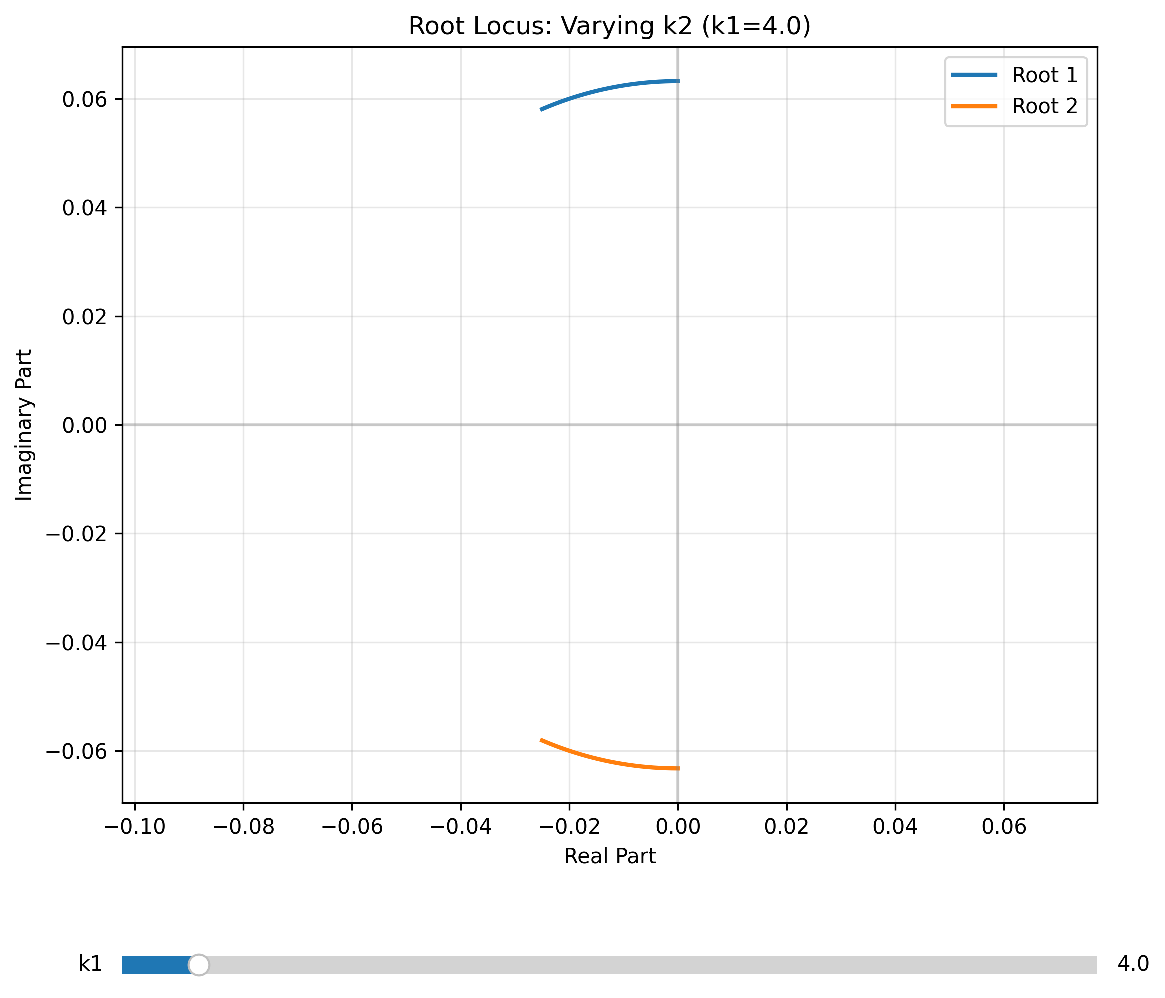
\includegraphics[width=\linewidth]{base_k2_root_locus(1).pdf}
        \caption{Fixed $k_1$}
        \label{fig:subfig2}
    \end{subfigure}
    \caption{Root Locus plots of manually input gains for large spacecraft case 1}
    \label{fig:combined}
\end{figure}
\end{frame}

% --- Small Spacecraft Results ---
\begin{frame}{Small Spacecraft Results - Time Domain \& Analysis}
    \begin{figure}[H]
    \label{Fig. 1}
    \centering
    \begin{subfigure}[b]{0.48\columnwidth}
        \label{Fig. 1.A}
        \centering
        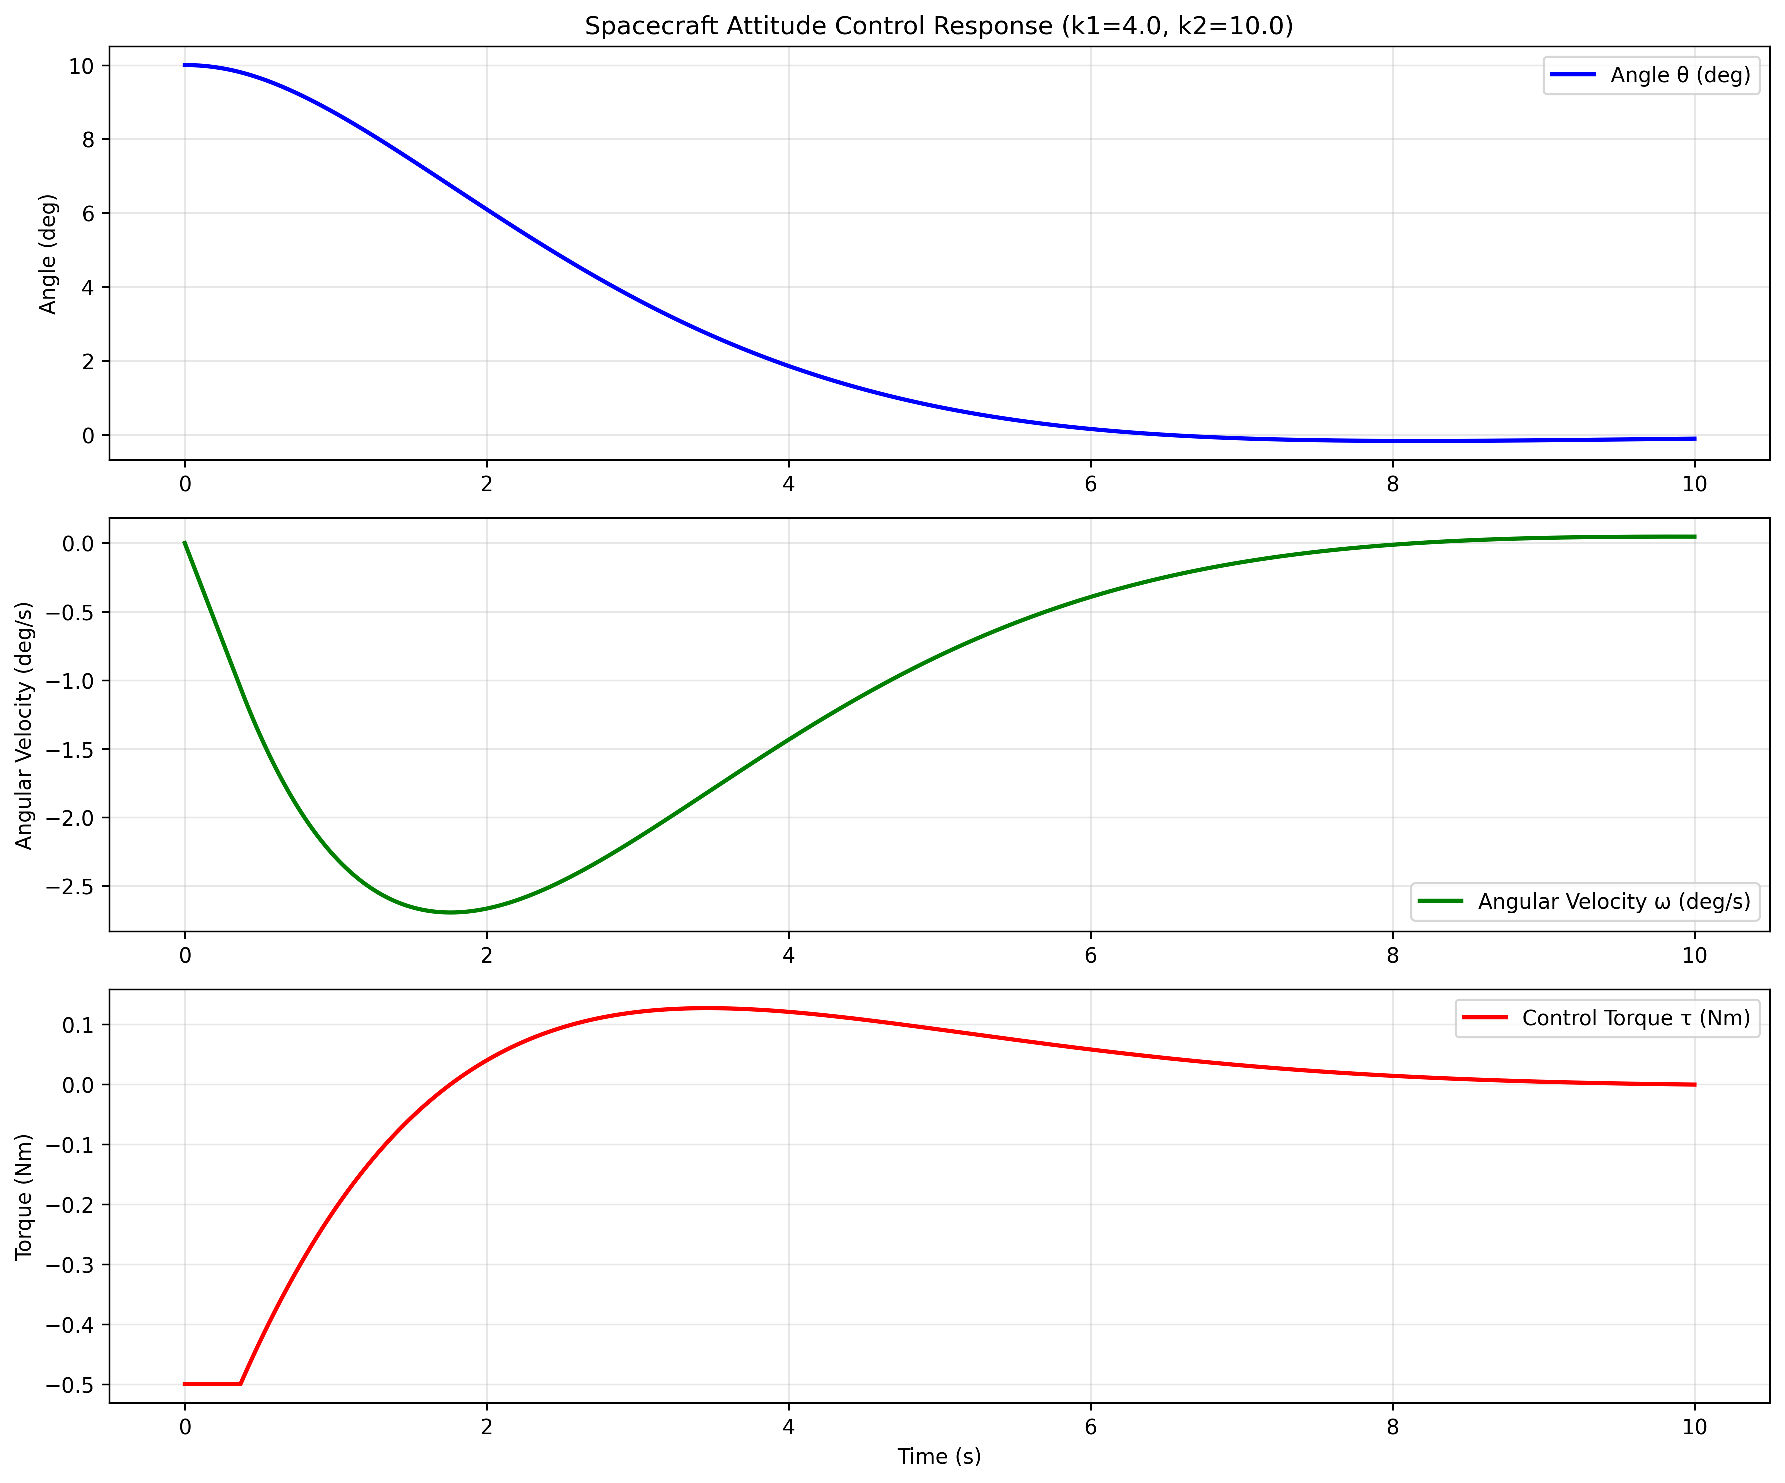
\includegraphics[width=\linewidth]{base_time_domain(4).pdf}
        \caption{Time-domain graphs}
        \label{fig:subfig1}
    \end{subfigure}
    \hfill
    \begin{subfigure}[b]{0.48\columnwidth}
        \label{Fig. 1.B}
        \centering
        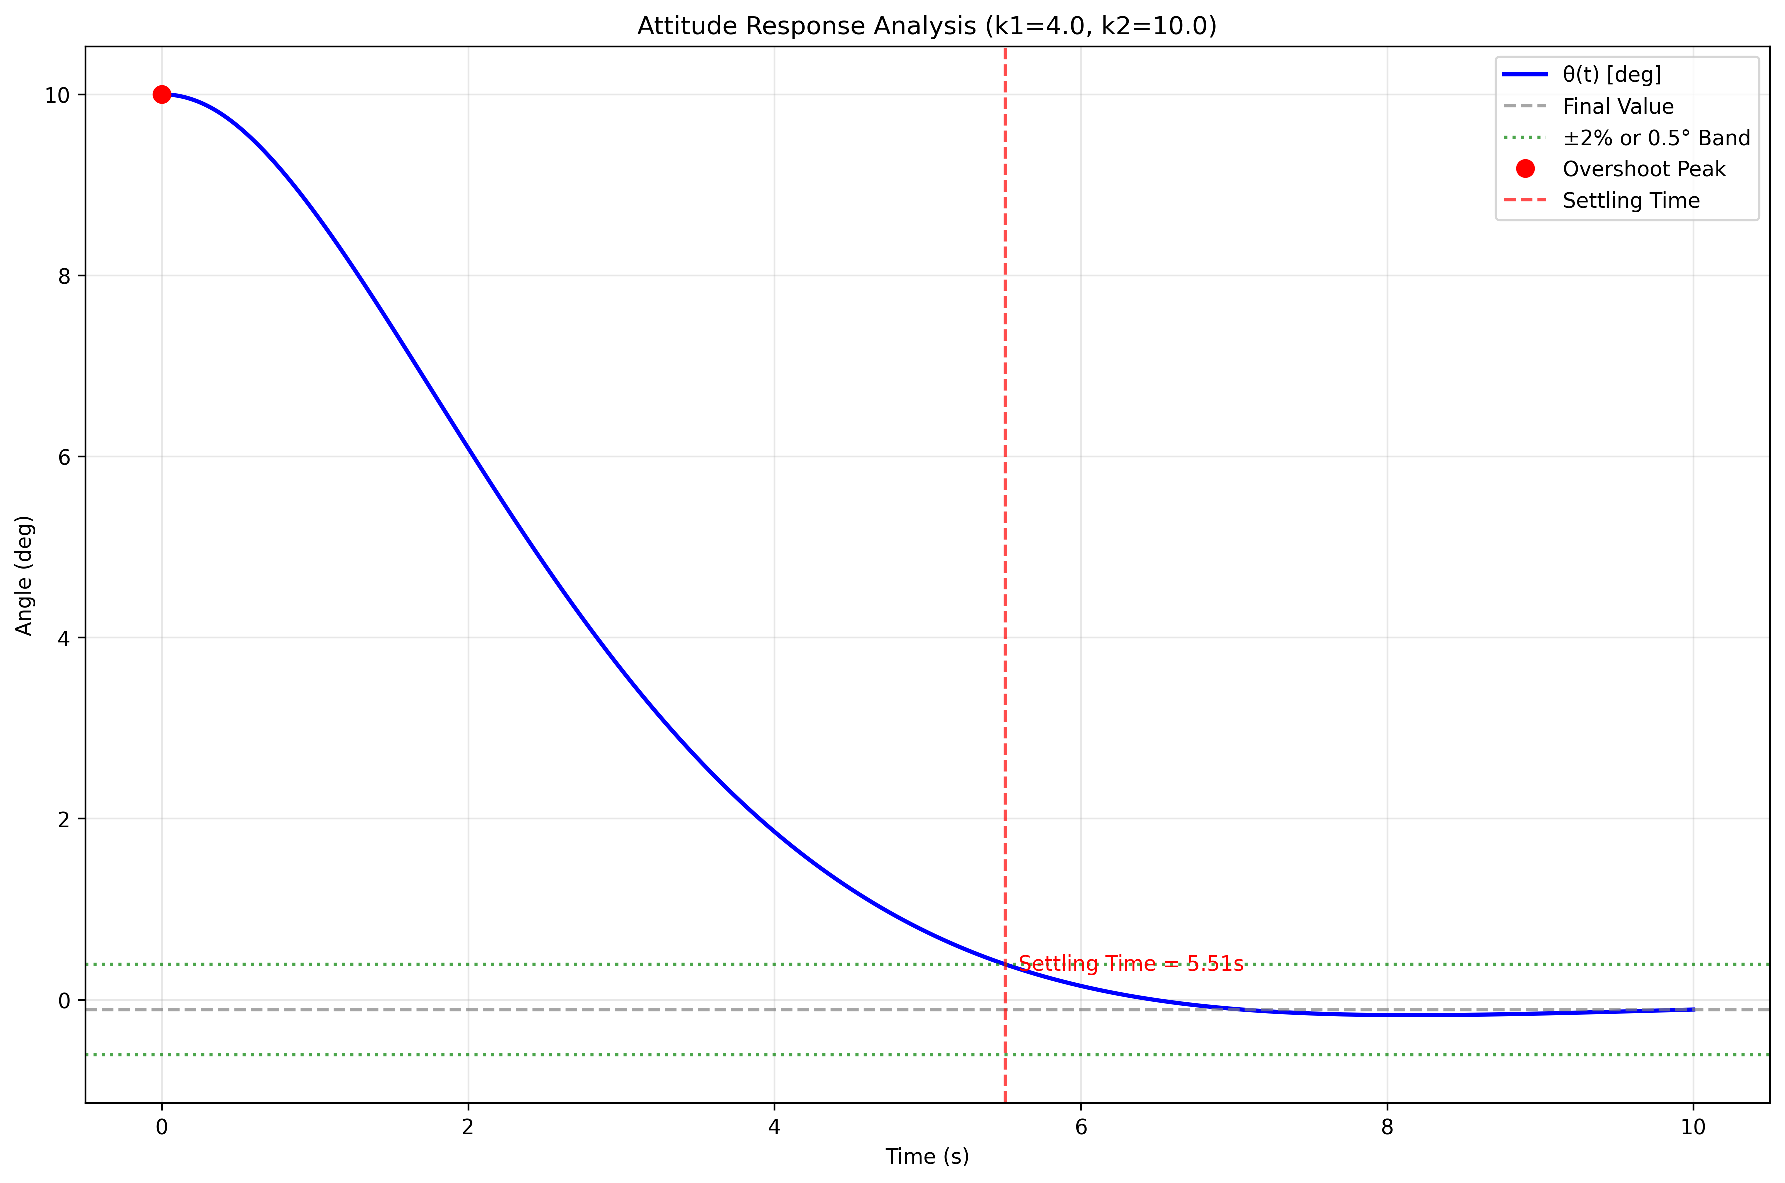
\includegraphics[width=\linewidth]{base_analysis(4).pdf}
        \caption{Response analysis graph}
        \label{fig:subfig2}
    \end{subfigure}
    \caption{Time-domain and Analysis of manually input gains for small spacecraft case 1}
    \label{fig:combined}
\end{figure}
\end{frame}

\begin{frame}{Small Spacecraft Results - Root Locus}
    \begin{figure}[H]
    \label{Fig. 1}
    \centering
    \begin{subfigure}[b]{0.48\columnwidth}
        \label{Fig. 1.A}
        \centering
        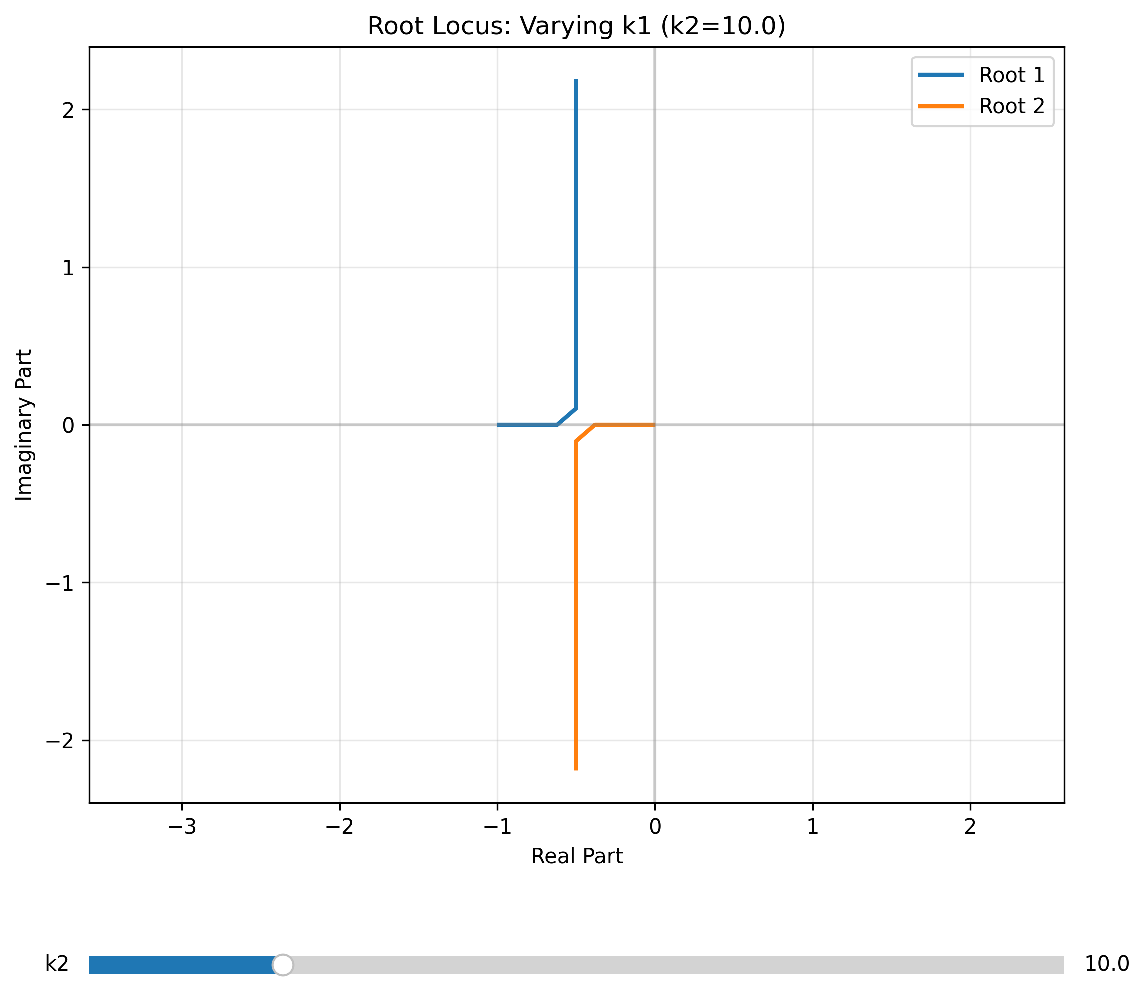
\includegraphics[width=\linewidth]{base_k1_root_locus(4).pdf}
        \caption{Fixed $k_1$}
        \label{fig:subfig1}
    \end{subfigure}
    \hfill
    \begin{subfigure}[b]{0.48\columnwidth}
        \label{Fig. 1.B}
        \centering
        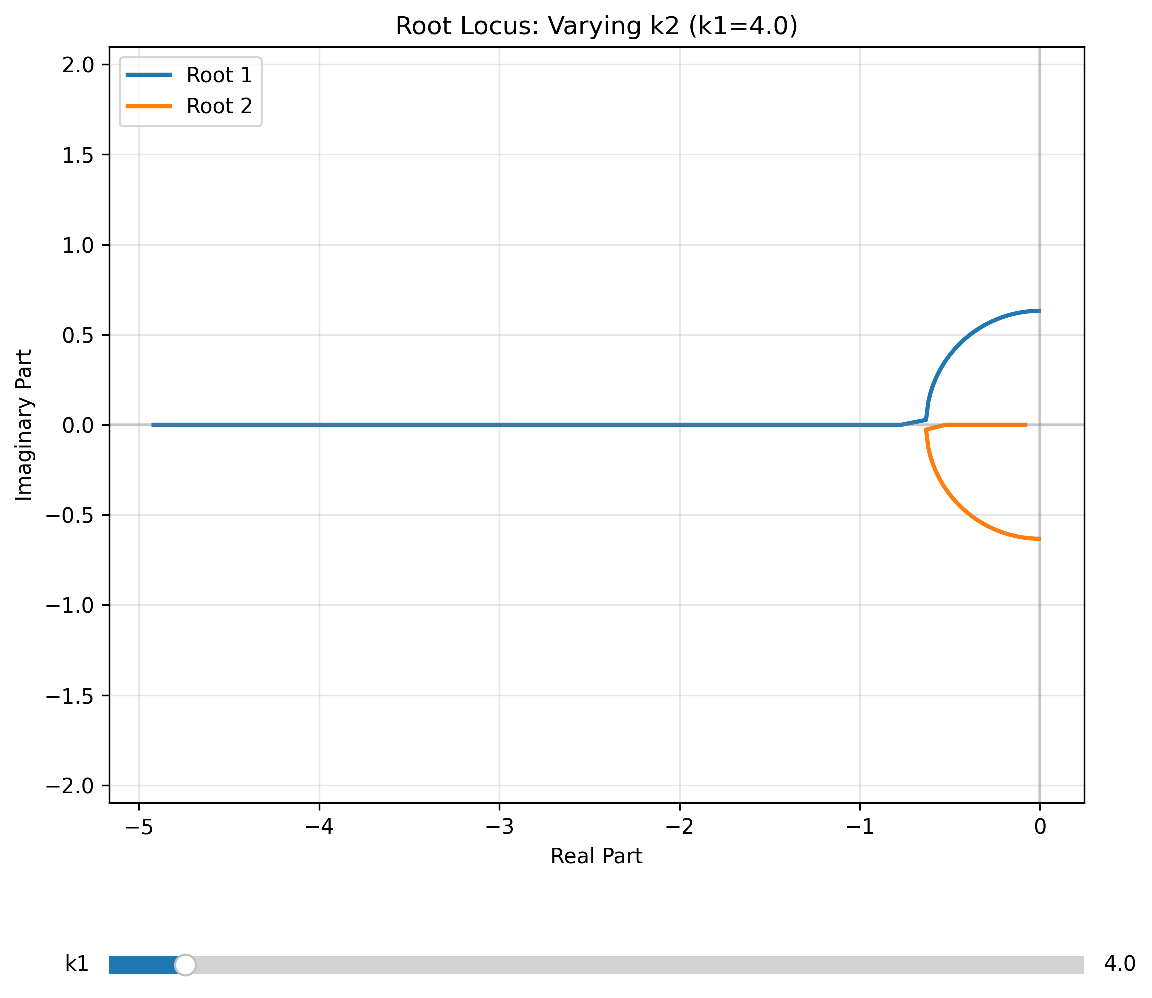
\includegraphics[width=\linewidth]{base_k2_root_locus(4).pdf}
        \caption{Fixed $k_2$}
        \label{fig:subfig2}
    \end{subfigure}
    \caption{Root Locus plots of manually input gains for small spacecraft case 1}
    \label{fig:combined}
\end{figure}
\end{frame}


% --- Cost Function ---
\section{Gain Optimization}
\begin{frame}{Gain Optimization Function}
    \begin{itemize}
        \item Estimate the most optimal range of gains
        \item Test gain combinations the resulting behavior
        \item Compare created gain combinations
    \end{itemize}
\end{frame}


\begin{frame}{Gain Optimization Cost Function}
\begin{itemize}
  \item Cost = weighted sum of:
  \begin{itemize}
    \item Settling time
    \item Overshoot
    \item Torque usage
  \end{itemize}
  \item Grid search across $(k_1, k_2)$ domain
  \item Select optimal gains that minimize cost
\end{itemize}
\end{frame}

% --- Grid Search Inefficiency ---

\begin{frame}{Gain Optimization Issues}
\begin{itemize}
  \item Failed to find valid optimal gains 
  \item Valid optimal gains found were skewed to the extreme of the range
\end{itemize}
\end{frame}

\begin{frame}{Gain Optimization Solution}
\begin{itemize}
  \item Created the estimate gains function
  \begin{itemize}
      \item Produced a range of possible gain based on the spacecraft dimensions
  \end{itemize}
\end{itemize}
\end{frame}

\begin{frame}{Program Inefficiency}
\begin{itemize}
  \item Uniform sampling: $200 \times 200 = 40{,}000$ combinations
  \item Inefficient in flat or highly sensitive regions
\end{itemize}
\end{frame}


\begin{frame}{Program Inefficiency - Solution}
\begin{itemize}
  \item ProcessPoolExecutor
  \item Gain estimation function reduced necessary values to loop over
  \item Reduced resolution for search from 100 $\longrightarrow$ 20
  \item Uniform sampling: $20 \times 20 = 400$ combinations
\end{itemize}
\end{frame}



\section{Comparison}

\begin{frame}{Large Spacecraft Results Comparison - Time-Domain}
    \begin{figure}[H]
    \label{Fig. 1}
    \centering
    \begin{subfigure}[b]{0.48\columnwidth}
        \label{Fig. 1.A}
        \centering
        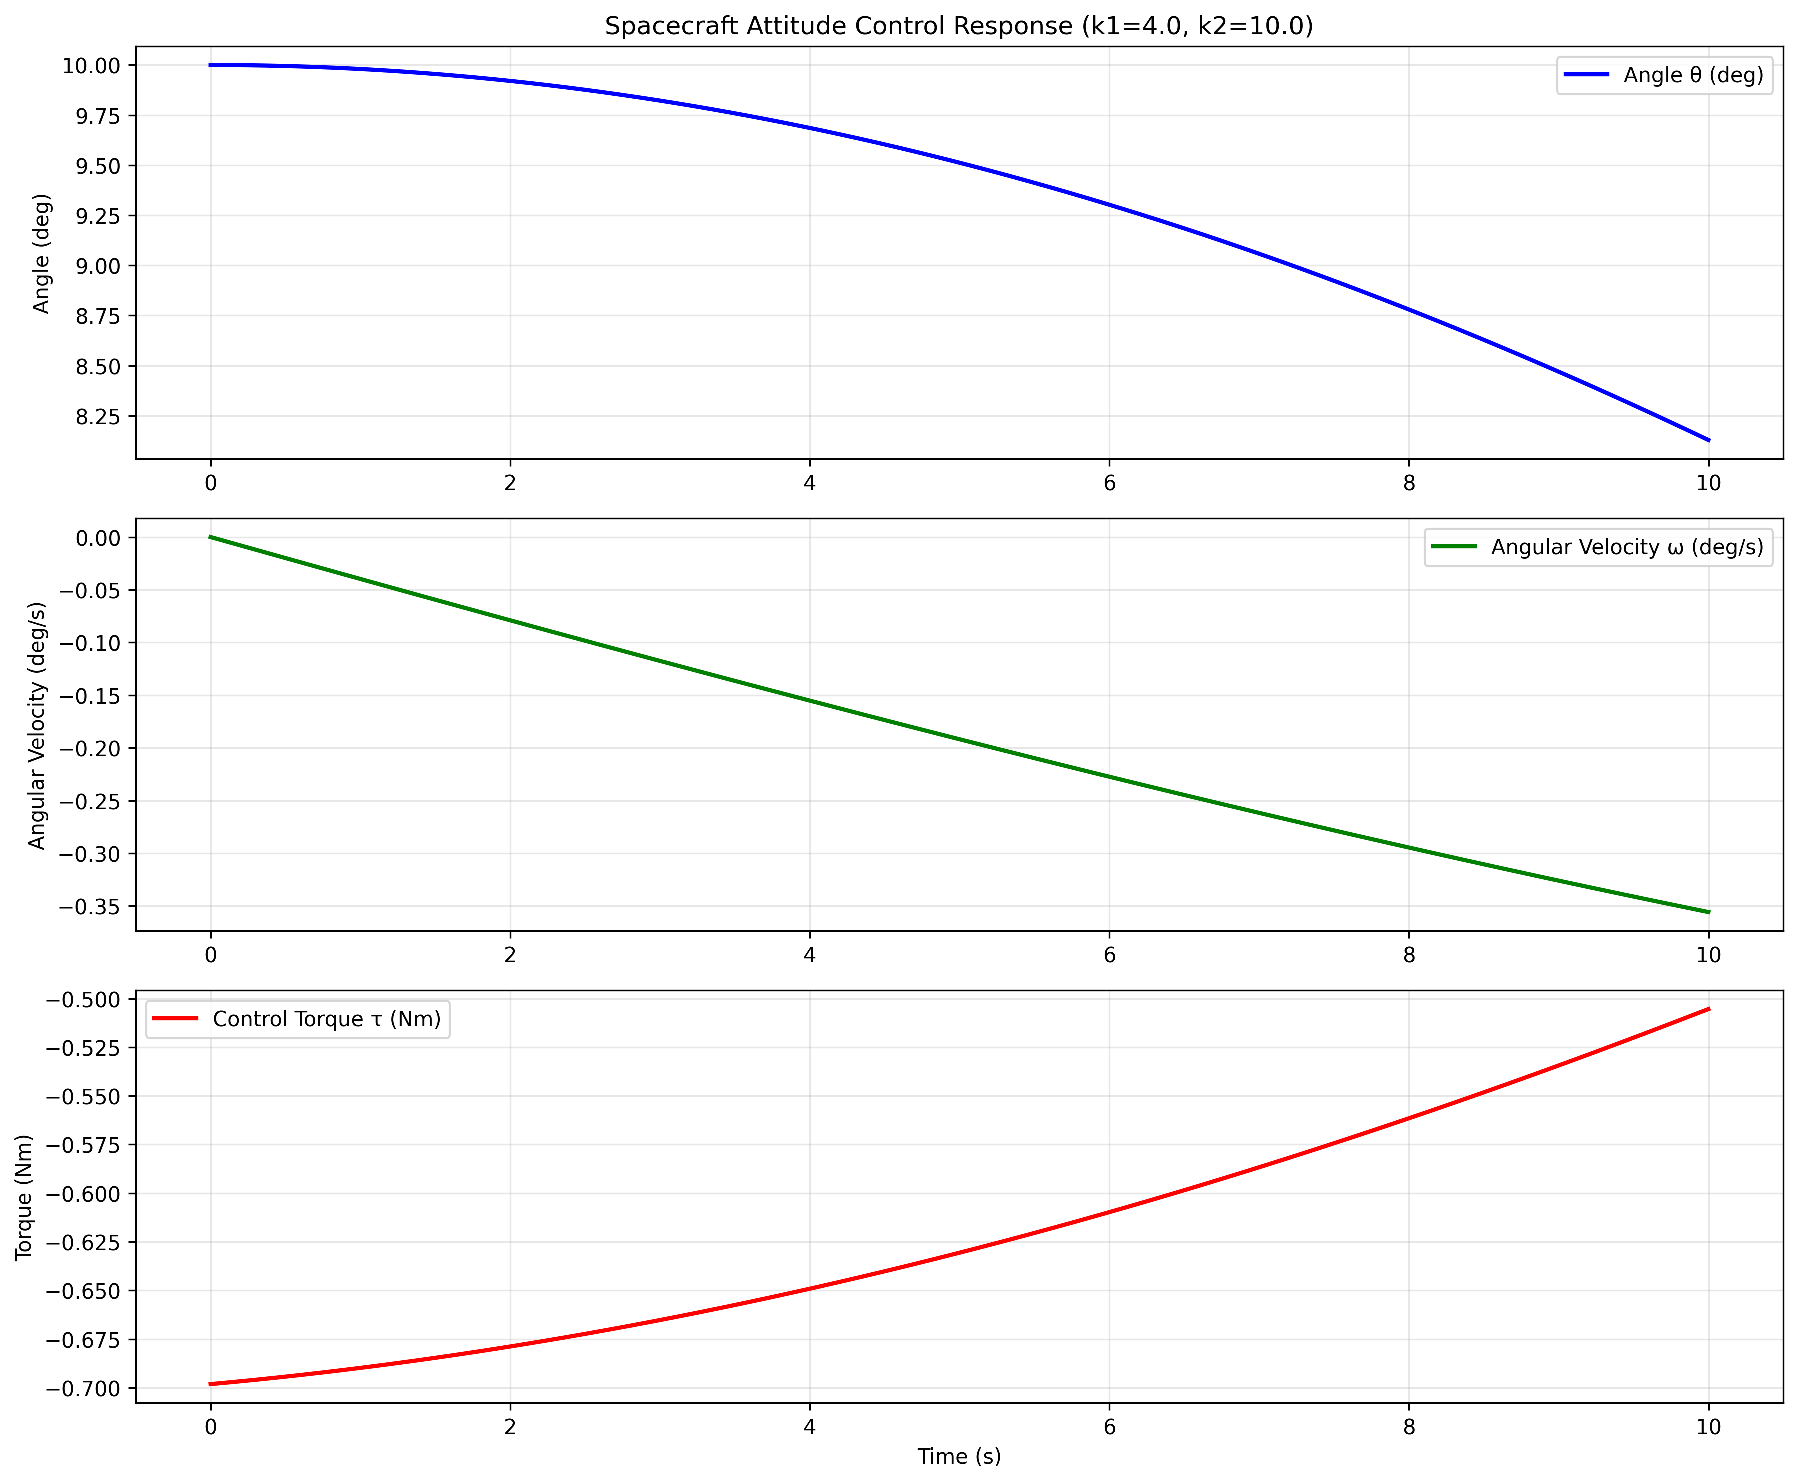
\includegraphics[width=\linewidth]{base_time_domain(1).pdf}
        \caption{Manually Input Gains}
        \label{fig:subfig1}
    \end{subfigure}
    \hfill
    \begin{subfigure}[b]{0.48\columnwidth}
        \label{Fig. 1.B}
        \centering
        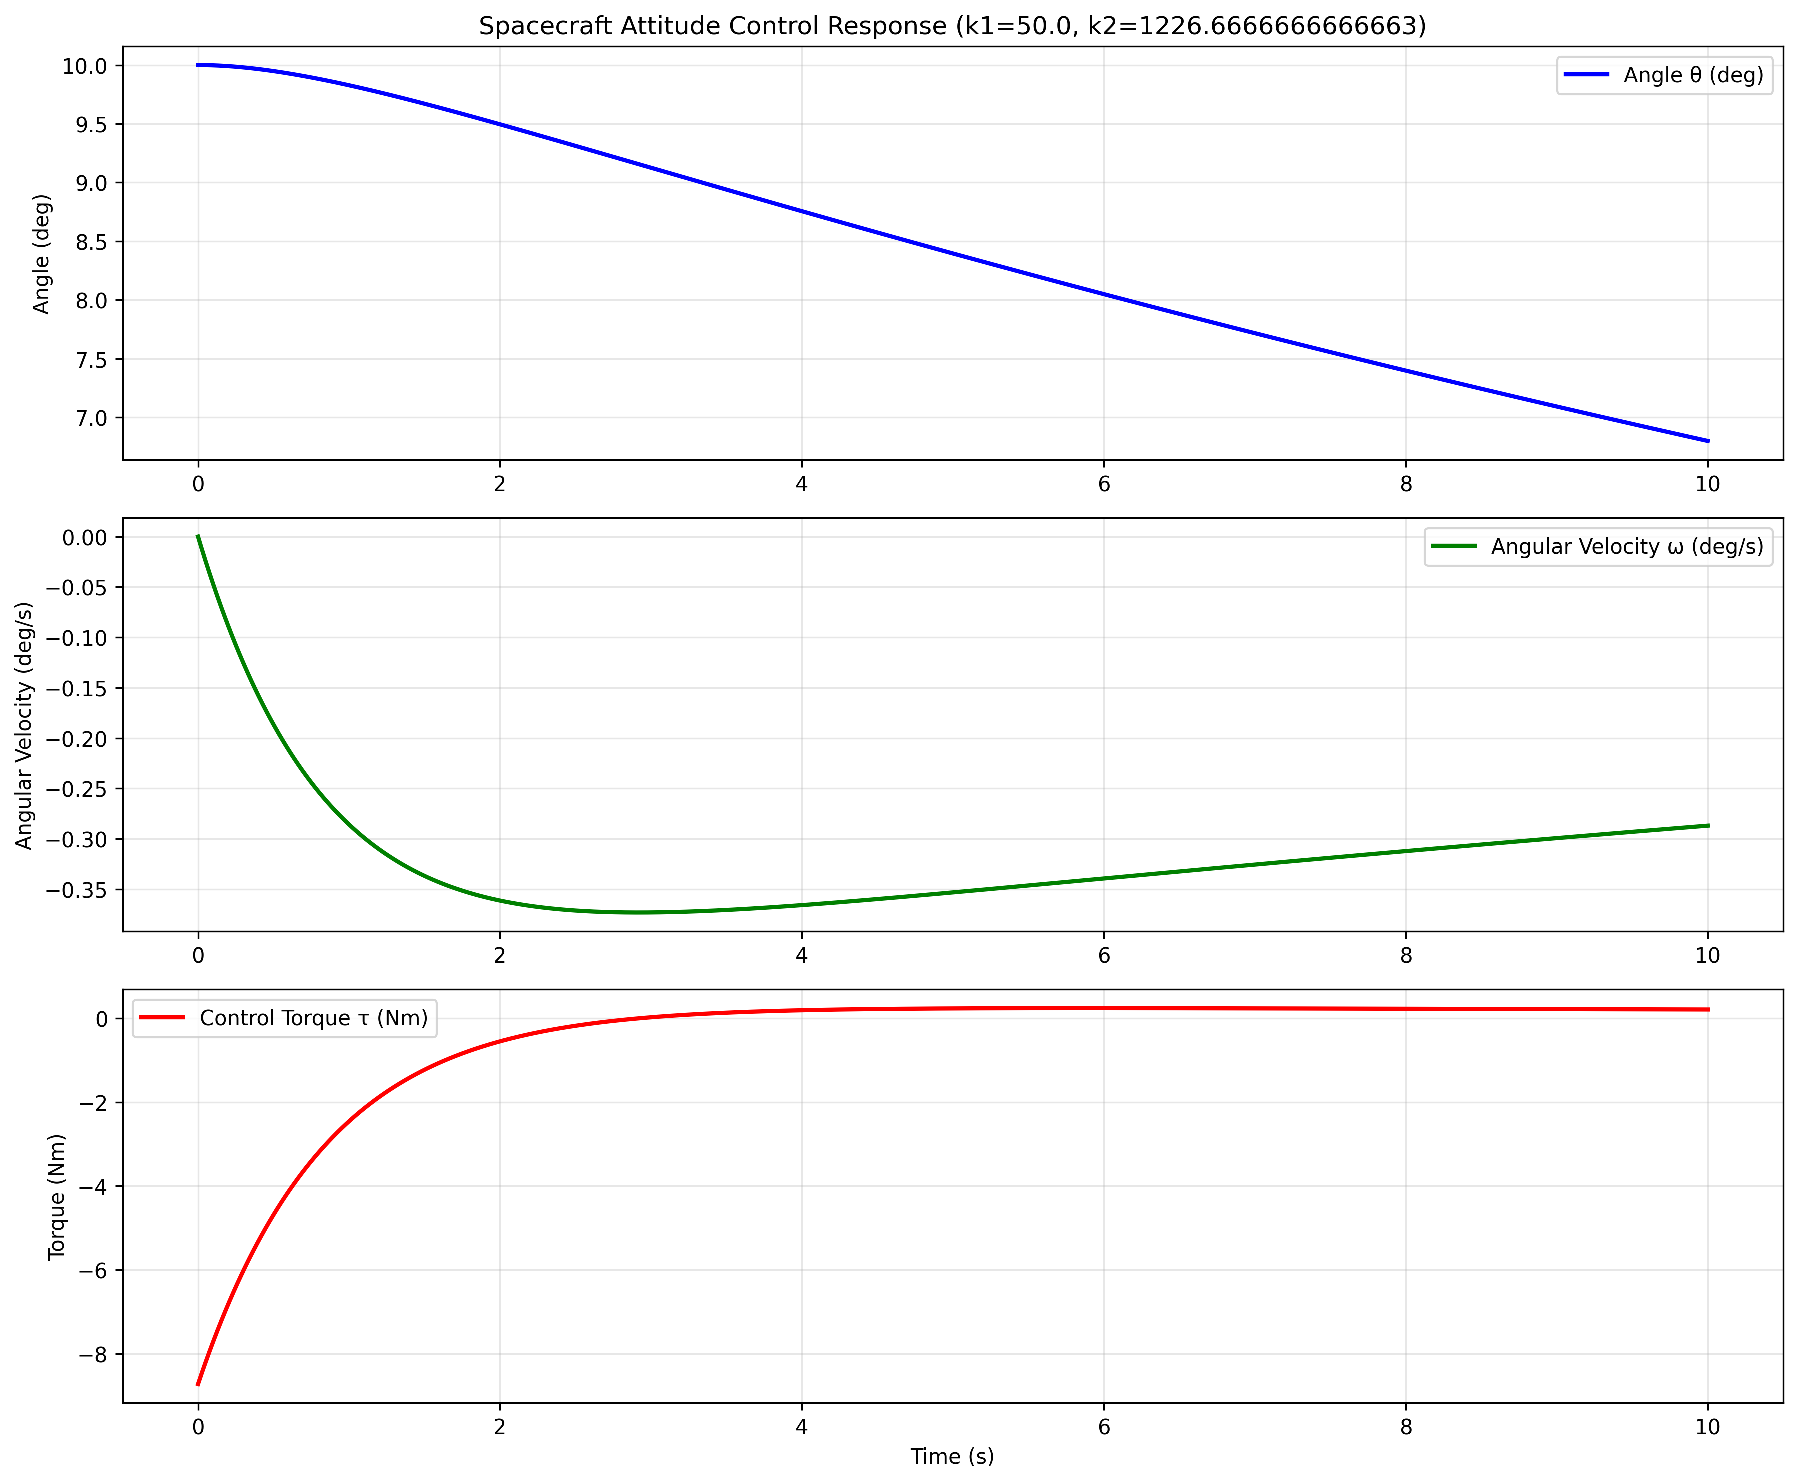
\includegraphics[width=\linewidth]{best_time_domain(1).pdf}
        \caption{Optomized Gains}
        \label{fig:subfig2}
    \end{subfigure}
    \caption{Time-domain graphs for large spacecraft case 1}
    \label{fig:combined}
\end{figure}
\end{frame}

\begin{frame}{Large Spacecraft Results Comparison - Analysis}
    \begin{figure}[H]
    \label{Fig. 1}
    \centering
    \begin{subfigure}[b]{0.48\columnwidth}
        \label{Fig. 1.A}
        \centering
        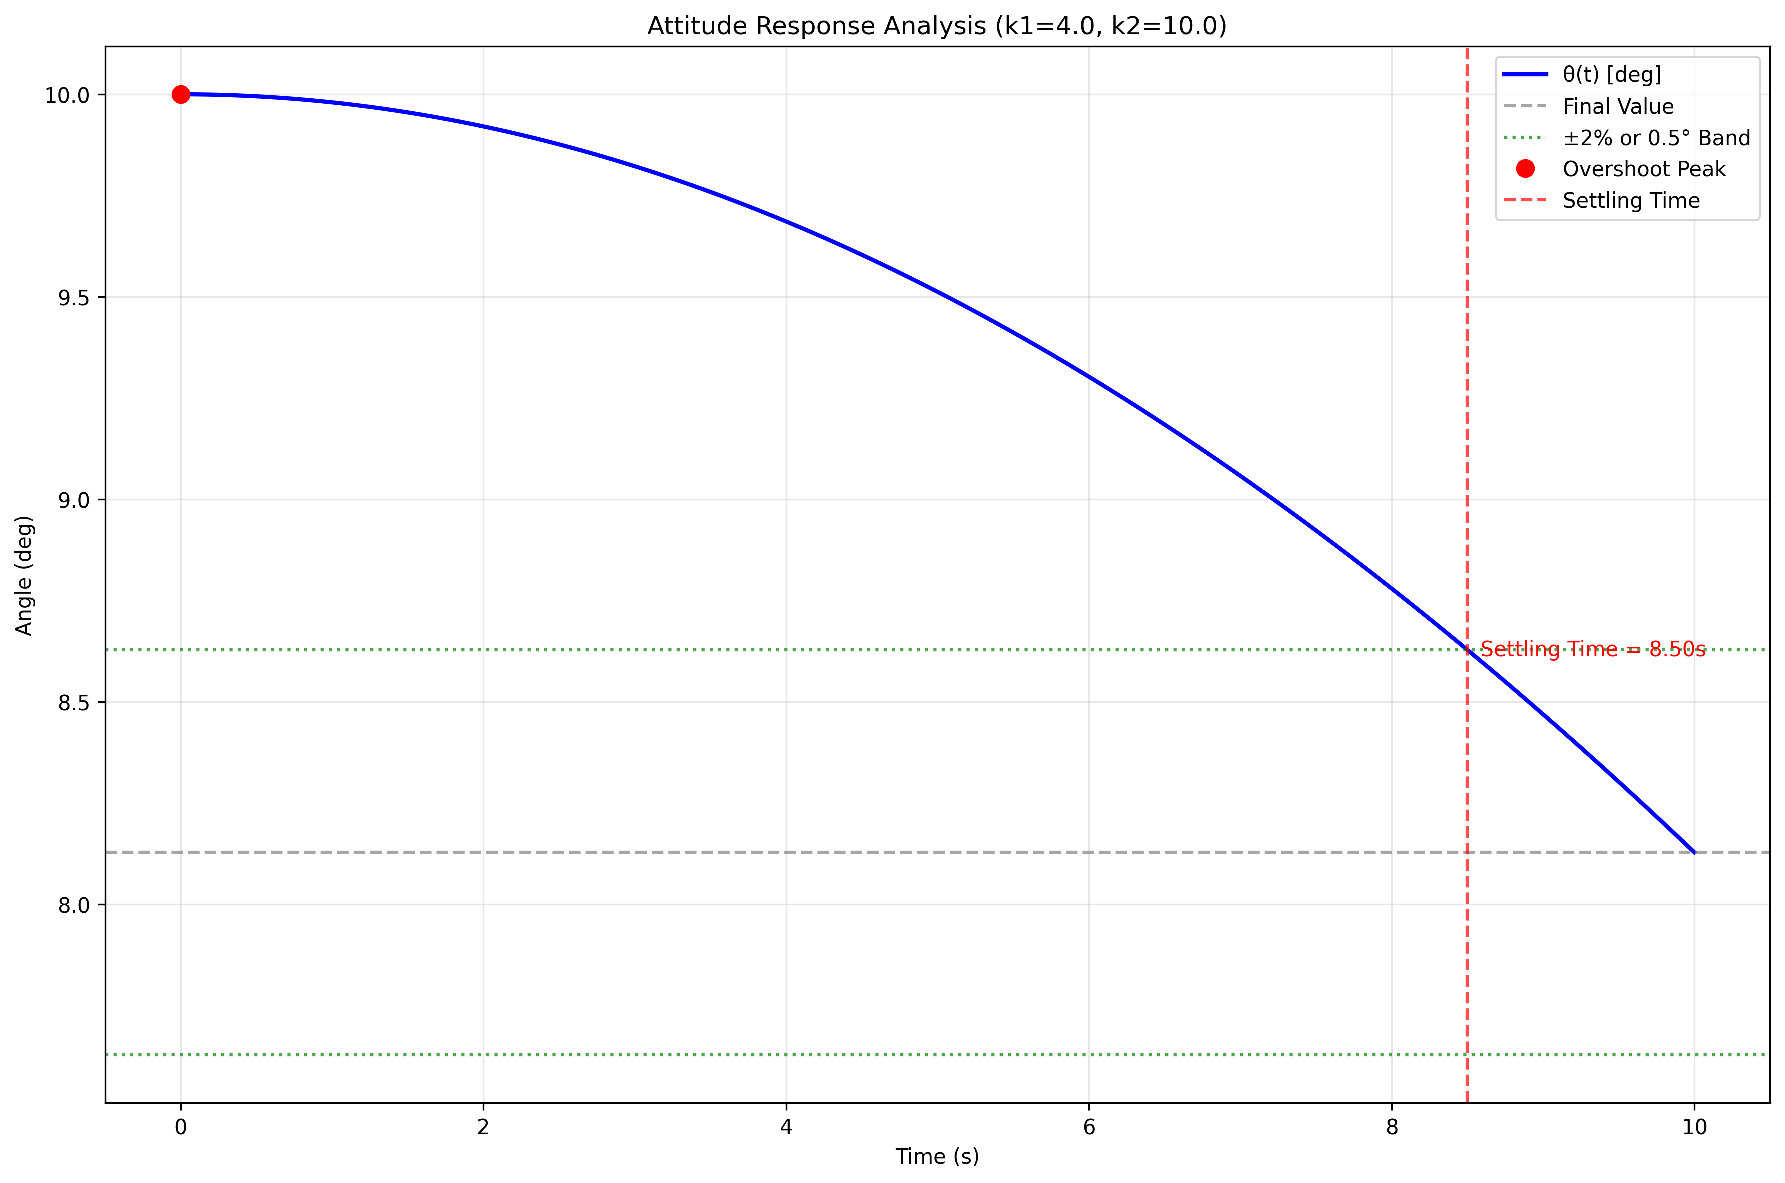
\includegraphics[width=\linewidth]{base_analysis(1).pdf}
        \caption{Manually Input Gains}
        \label{fig:subfig1}
    \end{subfigure}
    \hfill
    \begin{subfigure}[b]{0.48\columnwidth}
        \label{Fig. 1.B}
        \centering
        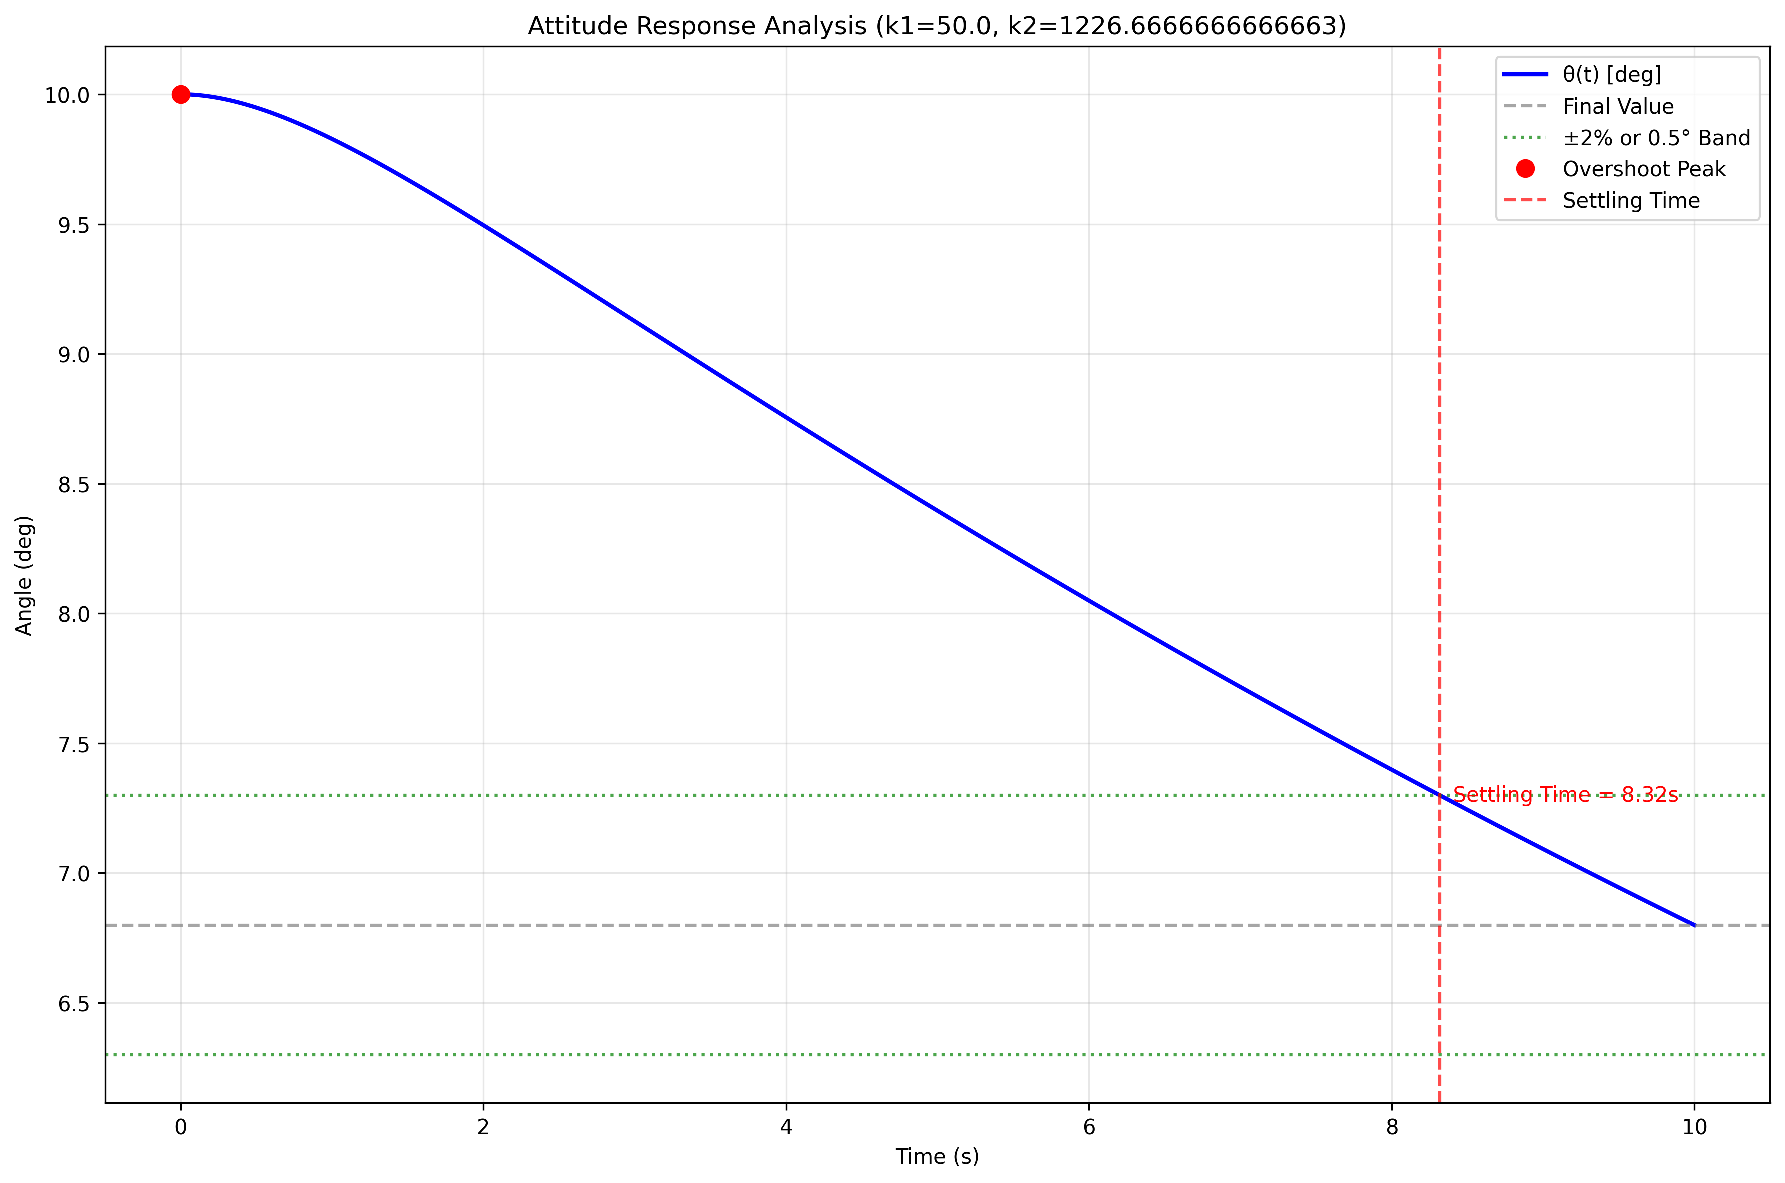
\includegraphics[width=\linewidth]{best_analysis(1).pdf}
        \caption{Optimized Gains}
        \label{fig:subfig2}
    \end{subfigure}
    \caption{Response Analysis graphs for large spacecraft case 1}
    \label{fig:combined}
\end{figure}
\end{frame}

\begin{frame}{Large Spacecraft Results Comparison - Root Locus($k_1$)}
    \begin{figure}[H]
    \label{Fig. 1}
    \centering
    \begin{subfigure}[b]{0.48\columnwidth}
        \label{Fig. 1.A}
        \centering
        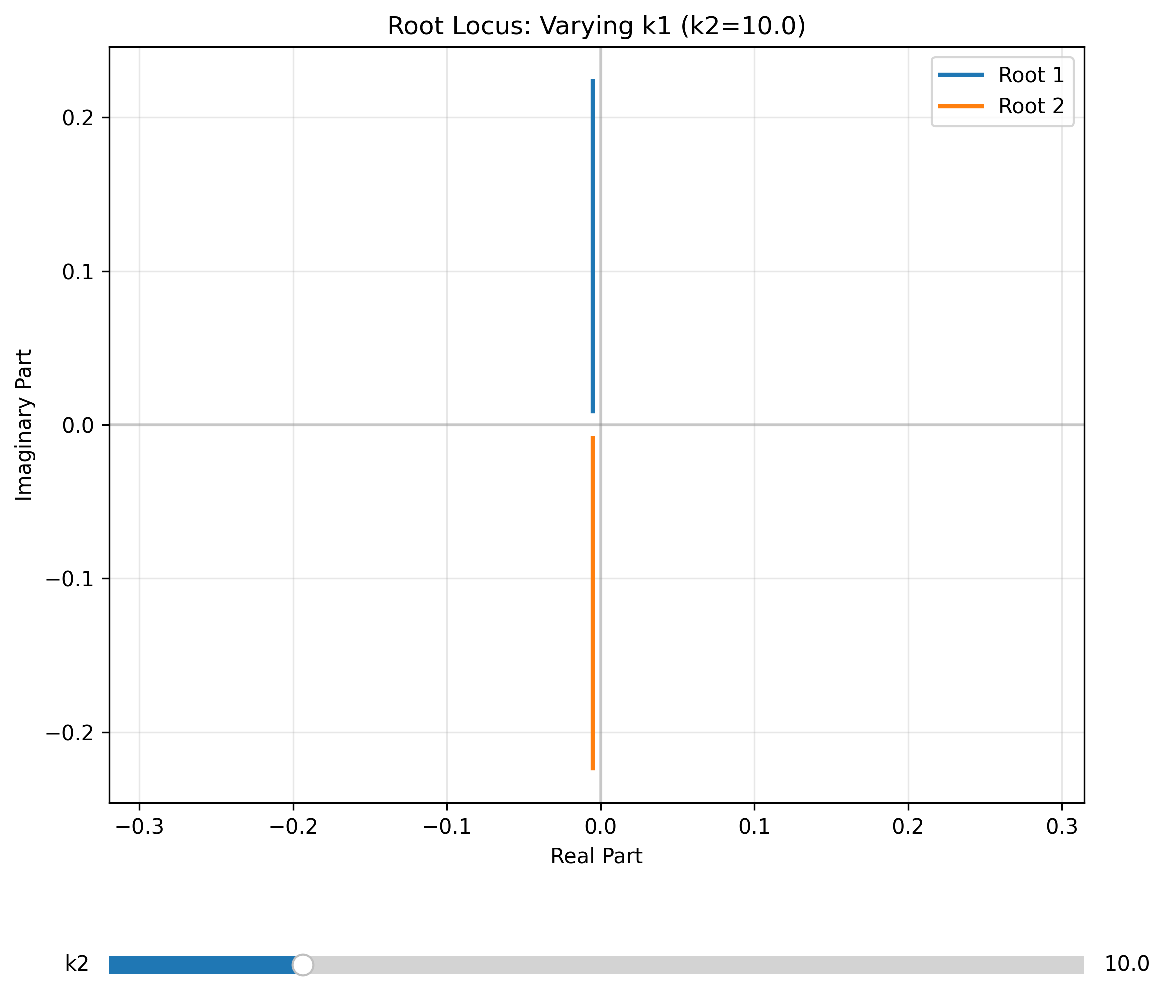
\includegraphics[width=\linewidth]{base_k1__root_locus(1).pdf}
        \caption{Manually input gains}
        \label{fig:subfig1}
    \end{subfigure}
    \hfill
    \begin{subfigure}[b]{0.48\columnwidth}
        \label{Fig. 1.B}
        \centering
        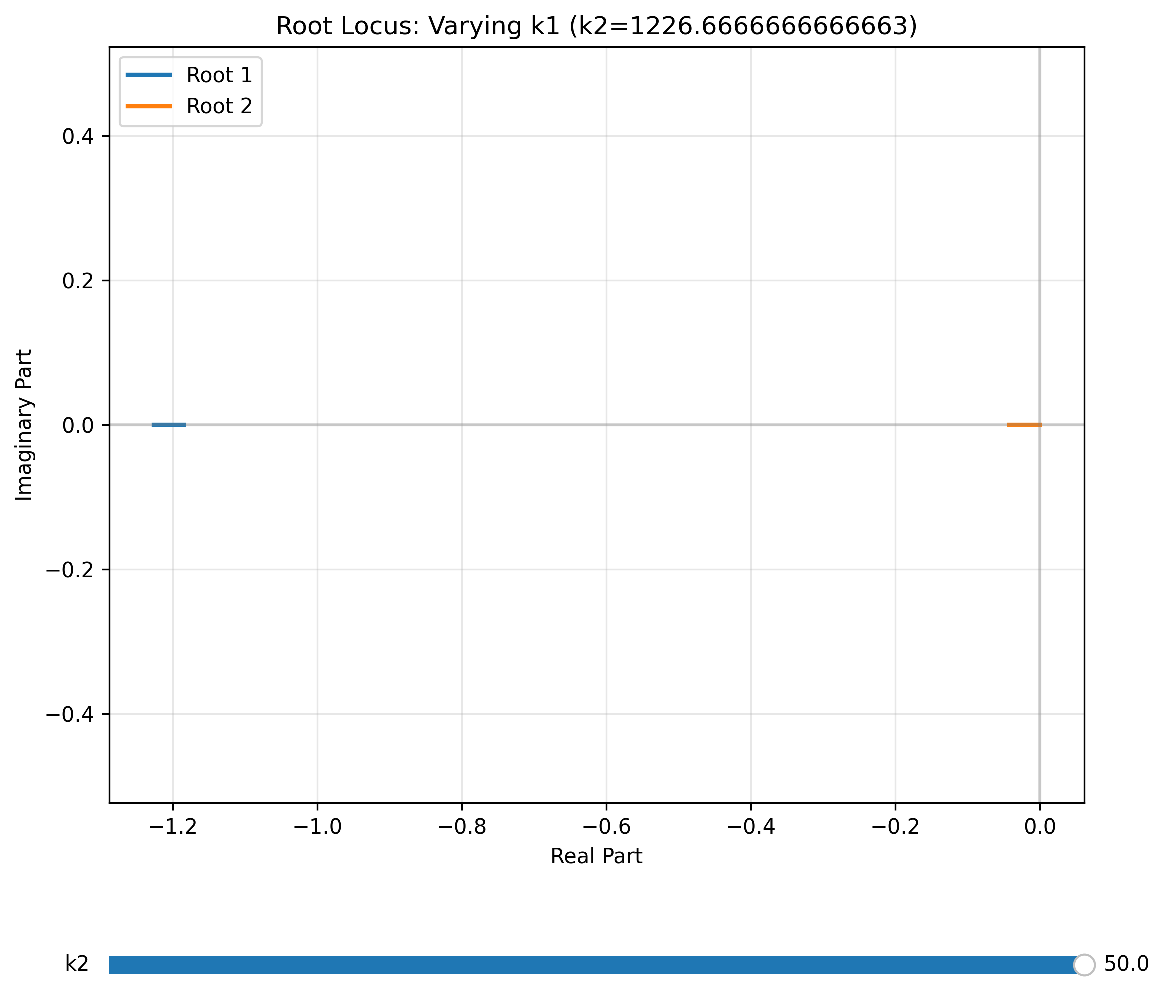
\includegraphics[width=\linewidth]{best_k1_root_locus(1).pdf}
        \caption{Optimized gains}
        \label{fig:subfig2}
    \end{subfigure}
    \caption{Root locus plots of a varying $k_1$ for large spacecraft case 1}
    \label{fig:combined}
\end{figure}
\end{frame}

\begin{frame}{Large Spacecraft Results Comparison - Root Locus($k_2$)}
    \begin{figure}[H]
    \label{Fig. 1}
    \centering
    \begin{subfigure}[b]{0.48\columnwidth}
        \label{Fig. 1.A}
        \centering
        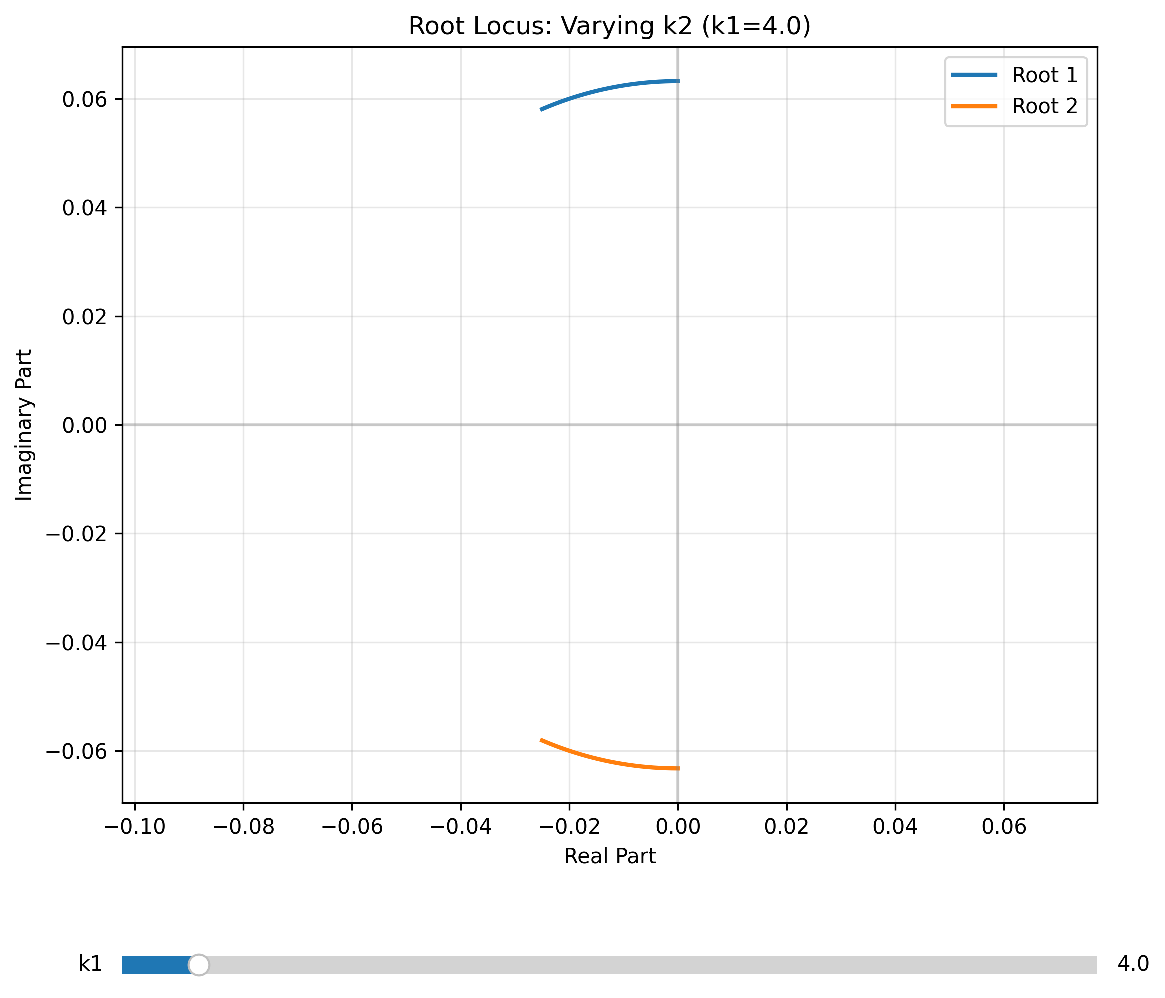
\includegraphics[width=\linewidth]{base_k2_root_locus(1).pdf}
        \caption{Manually input gains}
        \label{fig:subfig1}
    \end{subfigure}
    \hfill
    \begin{subfigure}[b]{0.48\columnwidth}
        \label{Fig. 1.B}
        \centering
        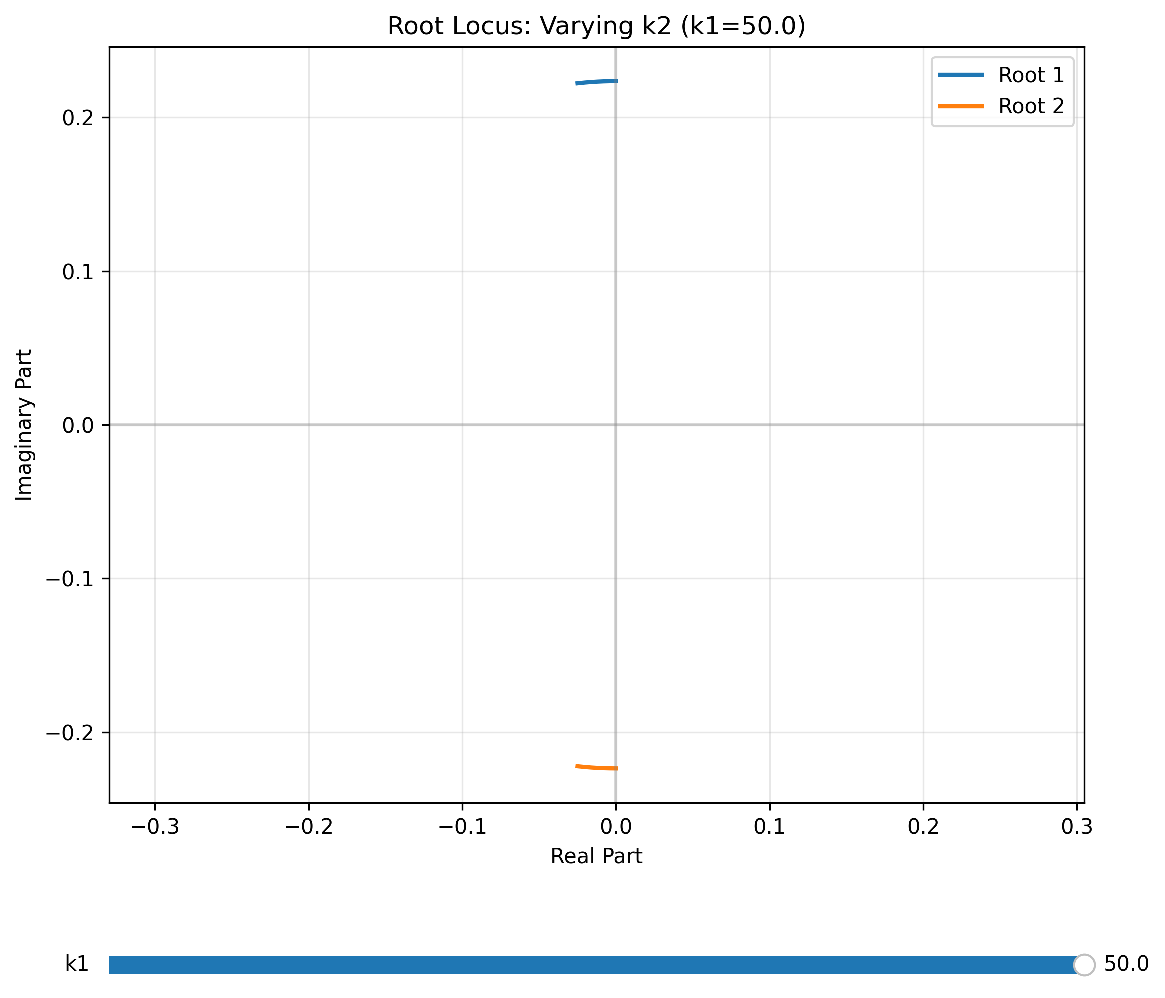
\includegraphics[width=\linewidth]{best_k2_root_locus(1).pdf}
        \caption{Optimized gains}
        \label{fig:subfig2}
    \end{subfigure}
    \caption{Root locus plots of a varying $k_2$ for large spacecraft case 1}
    \label{fig:combined}
\end{figure}
\end{frame}

\begin{frame}{Small Spacecraft Results Comparison - Time-Domain}
    \begin{figure}[H]
    \label{Fig. 1}
    \centering
    \begin{subfigure}[b]{0.48\columnwidth}
        \label{Fig. 1.A}
        \centering
        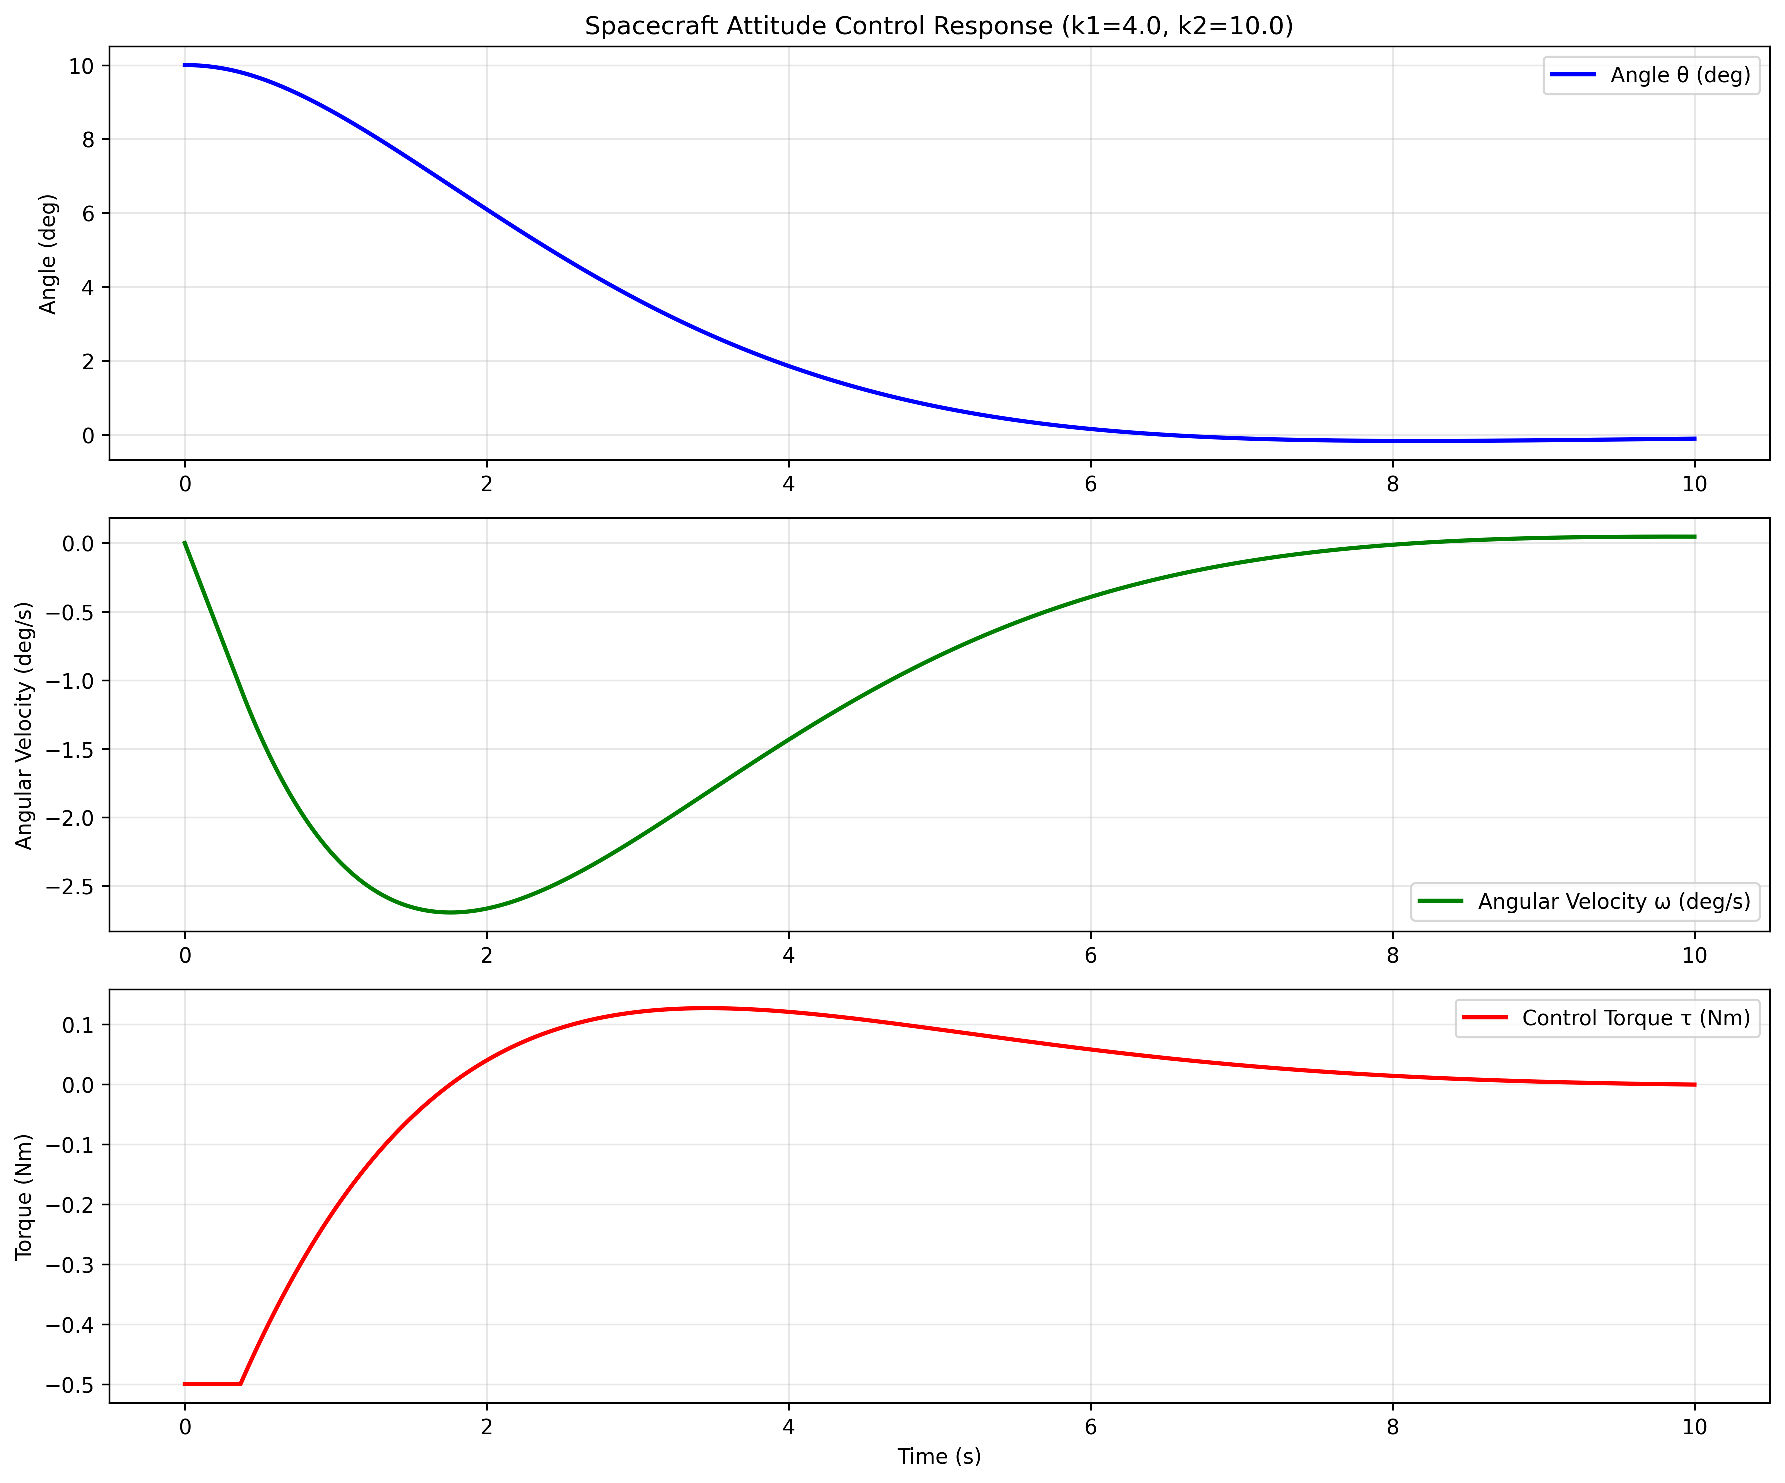
\includegraphics[width=\linewidth]{base_time_domain(4).pdf}
        \caption{Manually input gains}
        \label{fig:subfig1}
    \end{subfigure}
    \hfill
    \begin{subfigure}[b]{0.48\columnwidth}
        \label{Fig. 1.B}
        \centering
        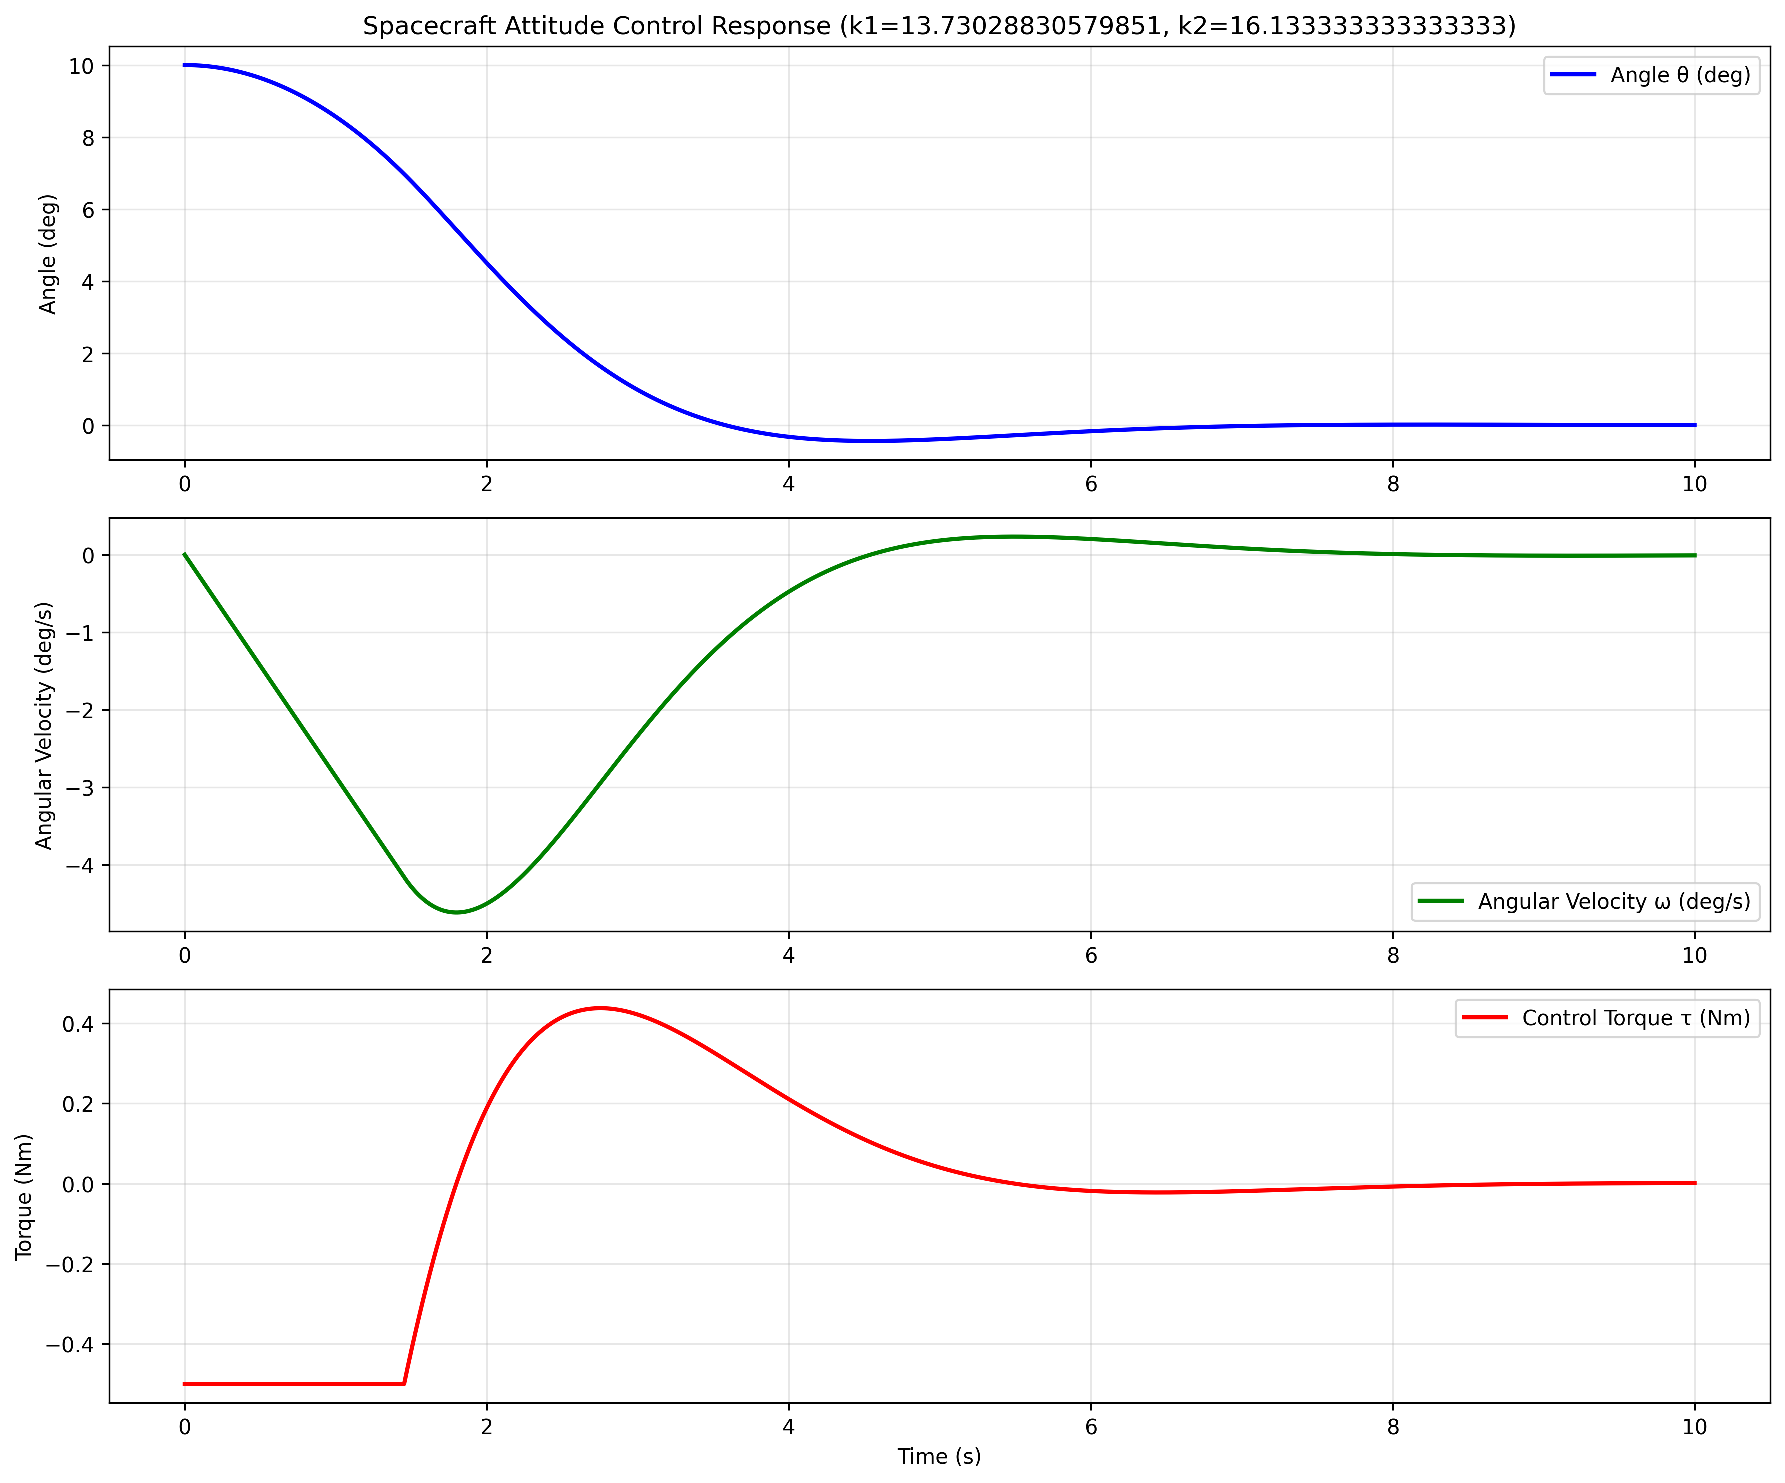
\includegraphics[width=\linewidth]{best_time_domain(4).pdf}
        \caption{Optimized gains}
        \label{fig:subfig2}
    \end{subfigure}
    \caption{Time-domain graphs for small spacecraft case 1}
    \label{fig:combined}
\end{figure}
\end{frame}

\begin{frame}{Small Spacecraft Results Comparison - Response Analysis}
    \begin{figure}[H]
    \label{Fig. 1}
    \centering
    \begin{subfigure}[b]{0.48\columnwidth}
        \label{Fig. 1.A}
        \centering
        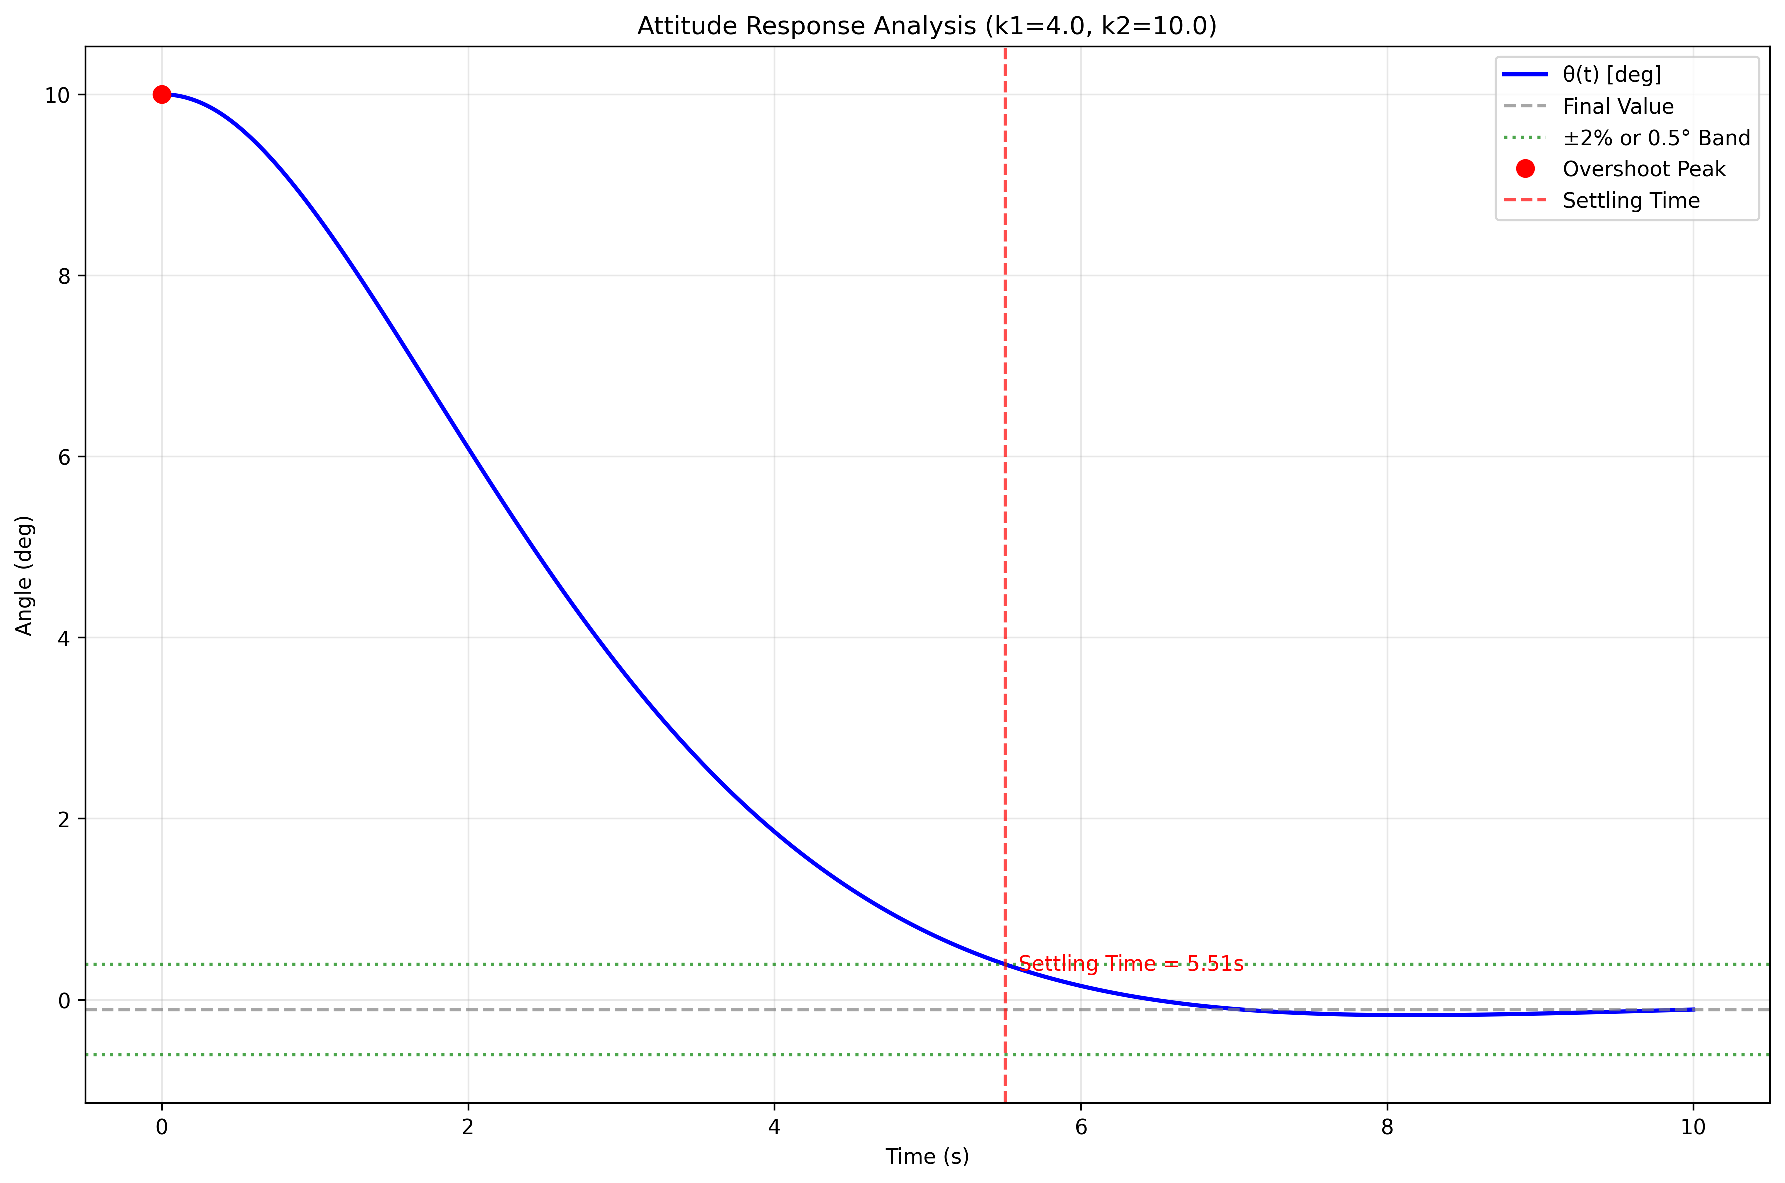
\includegraphics[width=\linewidth]{base_analysis(4).pdf}
        \caption{Manually input gains}
        \label{fig:subfig1}
    \end{subfigure}
    \hfill
    \begin{subfigure}[b]{0.48\columnwidth}
        \label{Fig. 1.B}
        \centering
        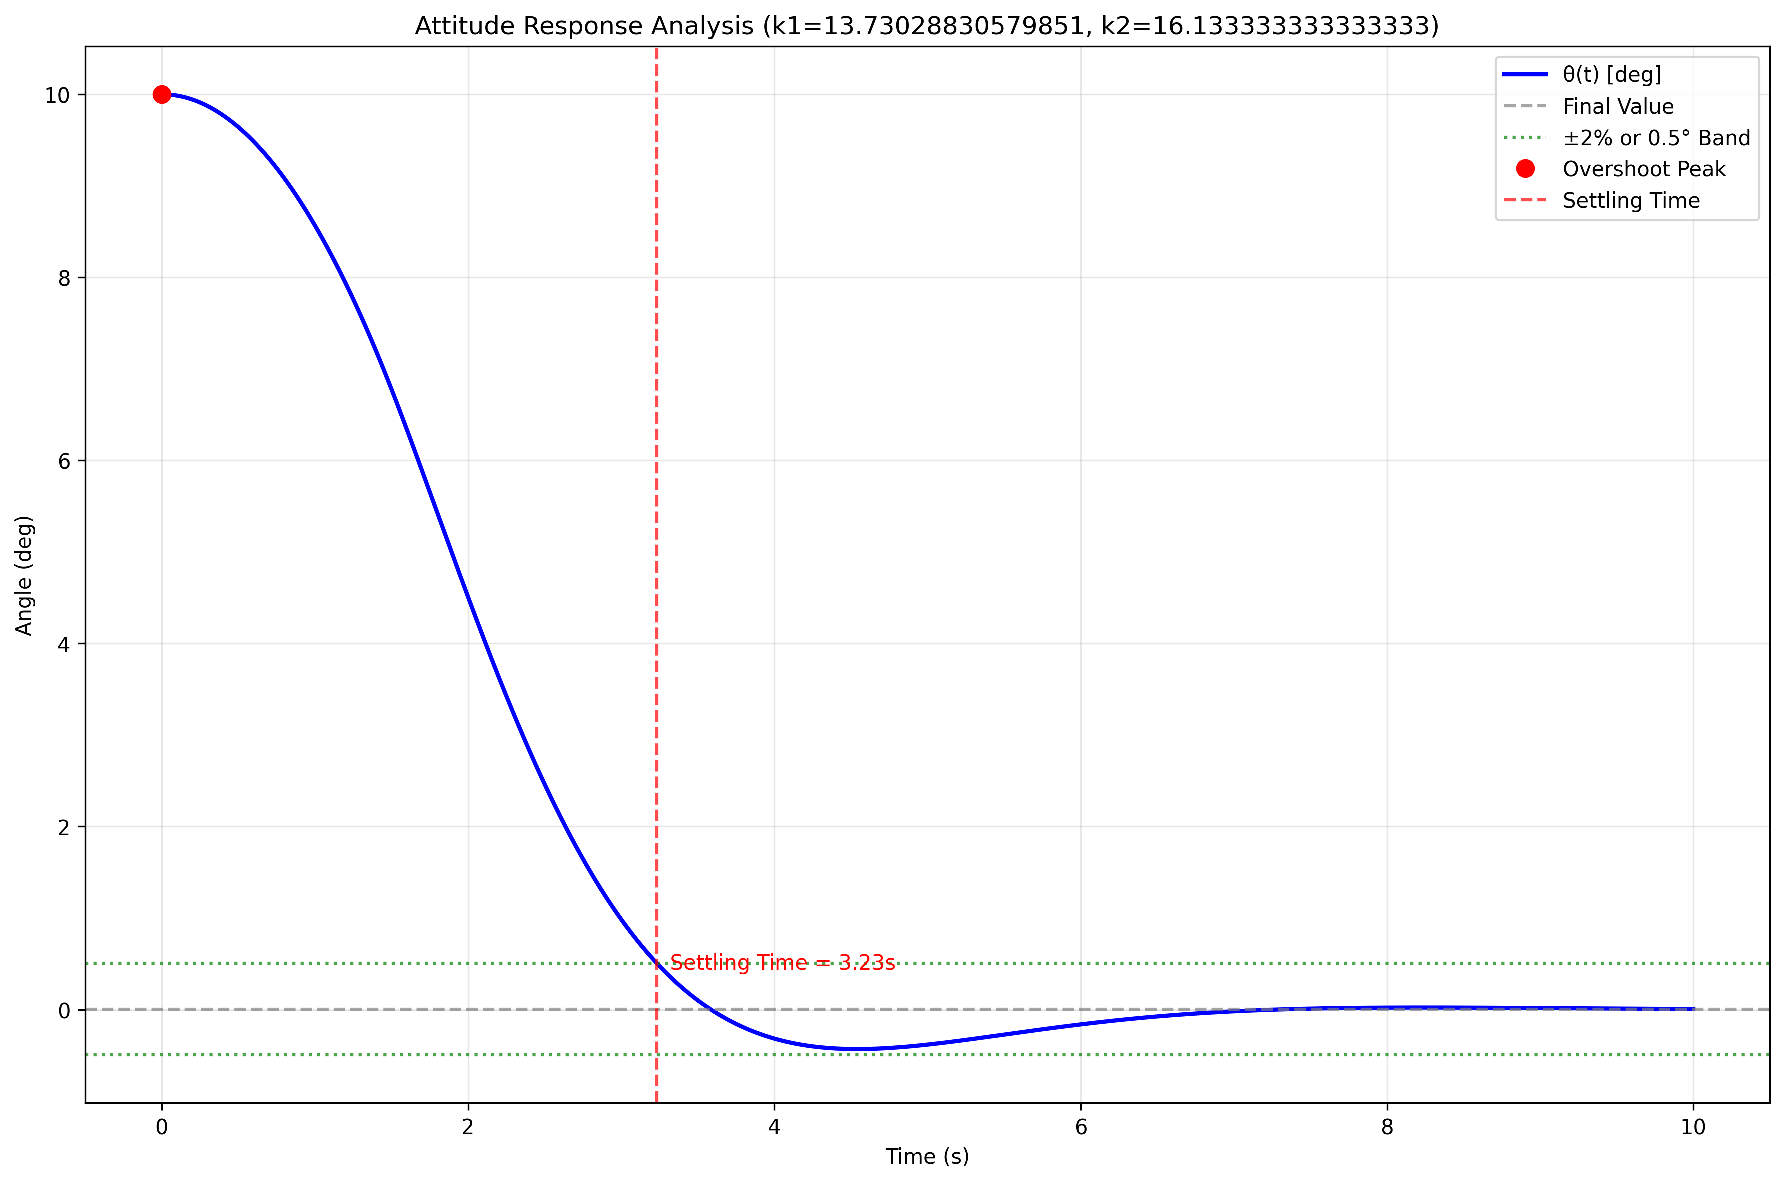
\includegraphics[width=\linewidth]{best_analysis(4).pdf}
        \caption{Optimized gains}
        \label{fig:subfig2}
    \end{subfigure}
    \caption{Response analysis graphs for small spacecraft case 1}
    \label{fig:combined}
\end{figure}
\end{frame}

\begin{frame}{Large Spacecraft Results Comparison - Root Locus ($k_1$)}
    \begin{figure}[H]
    \label{Fig. 1}
    \centering
    \begin{subfigure}[b]{0.48\columnwidth}
        \label{Fig. 1.A}
        \centering
        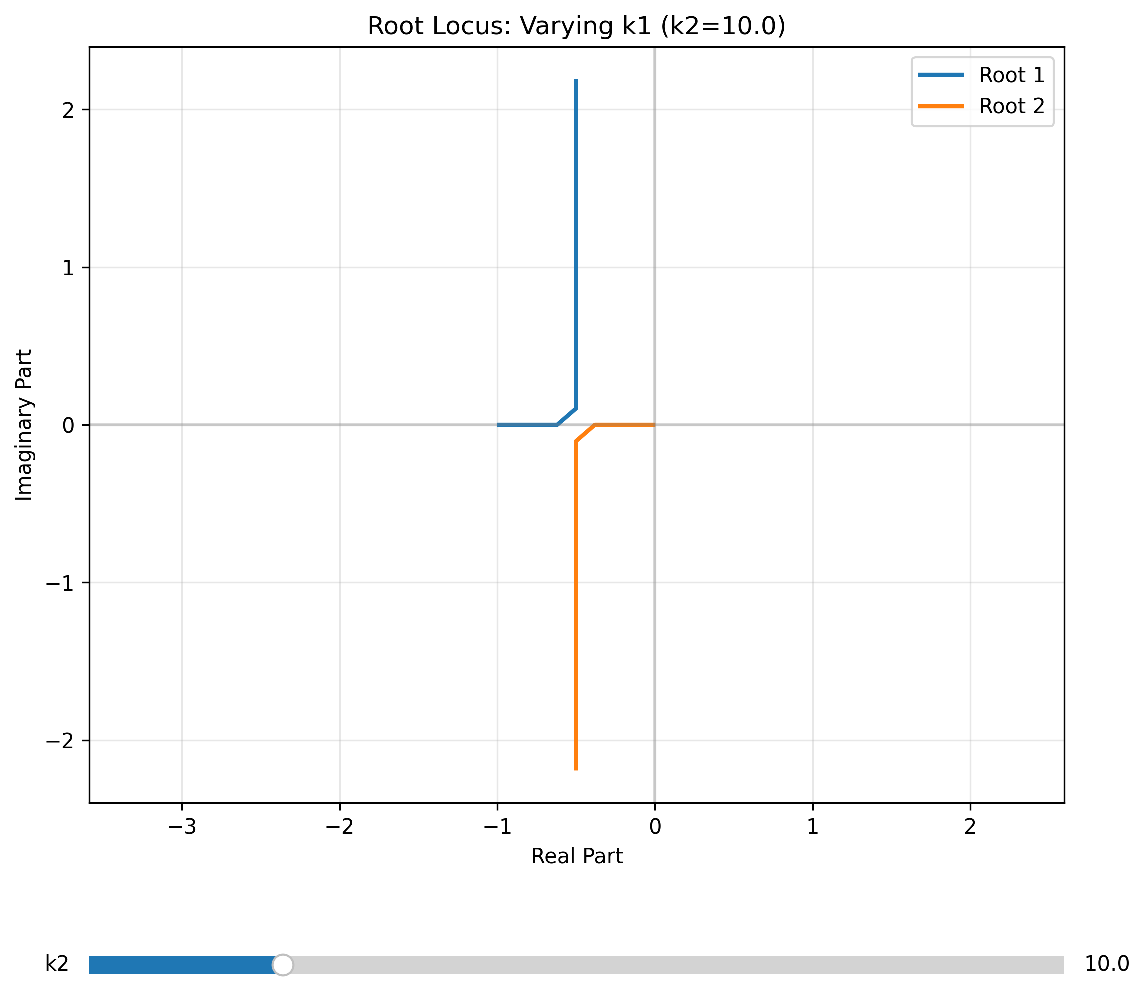
\includegraphics[width=\linewidth]{base_k1_root_locus(4).pdf}
        \caption{Manually input gains}
        \label{fig:subfig1}
    \end{subfigure}
    \hfill
    \begin{subfigure}[b]{0.48\columnwidth}
        \label{Fig. 1.B}
        \centering
        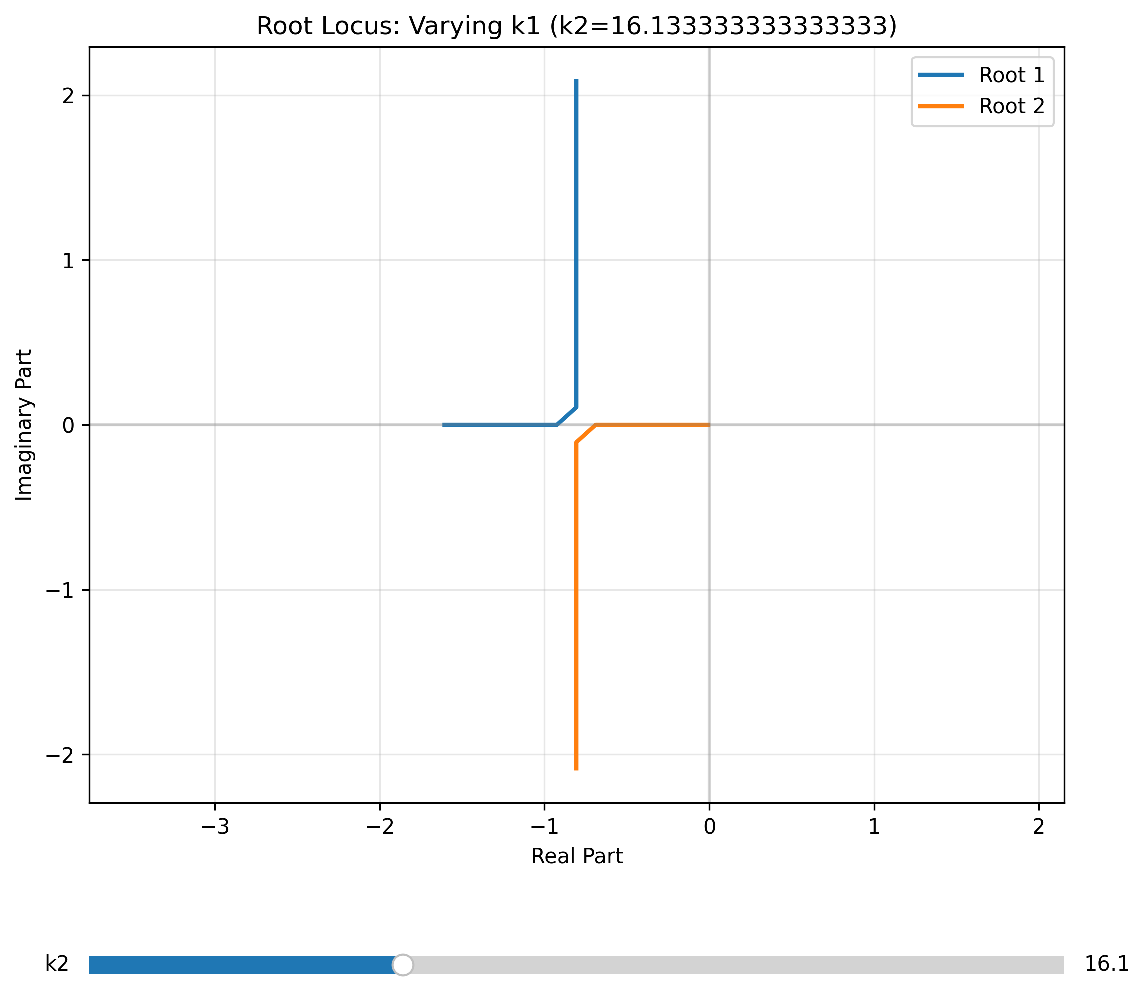
\includegraphics[width=\linewidth]{best_k1_root_locus(4).pdf}
        \caption{Optimized gains}
        \label{fig:subfig2}
    \end{subfigure}
    \caption{Root locus plots for a varying $k_1$ of small spacecraft case 1}
    \label{fig:combined}
\end{figure}
\end{frame}

\begin{frame}{Large Spacecraft Results Comparison - Root Locus ($k_2$)}
    \begin{figure}[H]
    \label{Fig. 1}
    \centering
    \begin{subfigure}[b]{0.48\columnwidth}
        \label{Fig. 1.A}
        \centering
        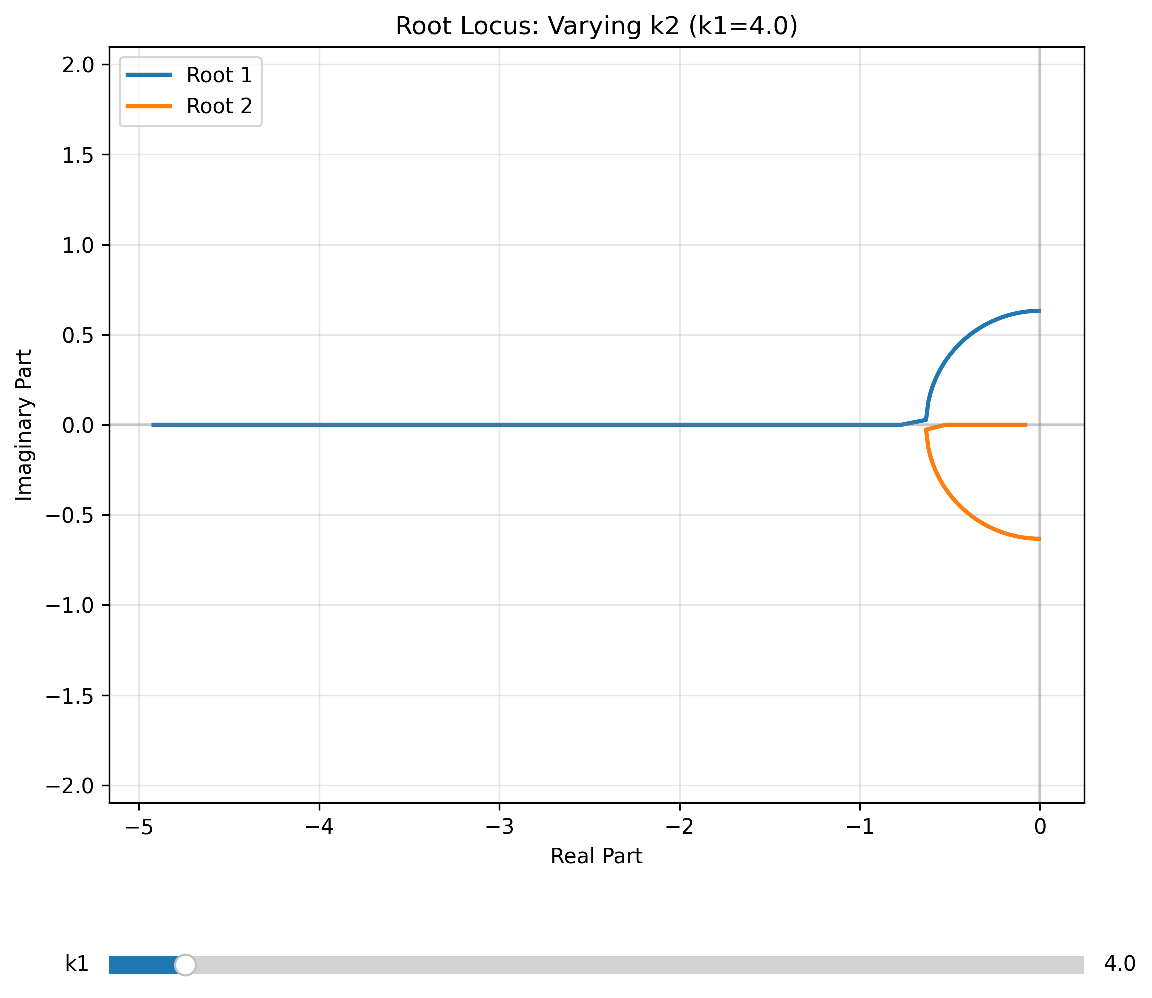
\includegraphics[width=\linewidth]{base_k2_root_locus(4).pdf}
        \caption{Manually input gains}
        \label{fig:subfig1}
    \end{subfigure}
    \hfill
    \begin{subfigure}[b]{0.48\columnwidth}
        \label{Fig. 1.B}
        \centering
        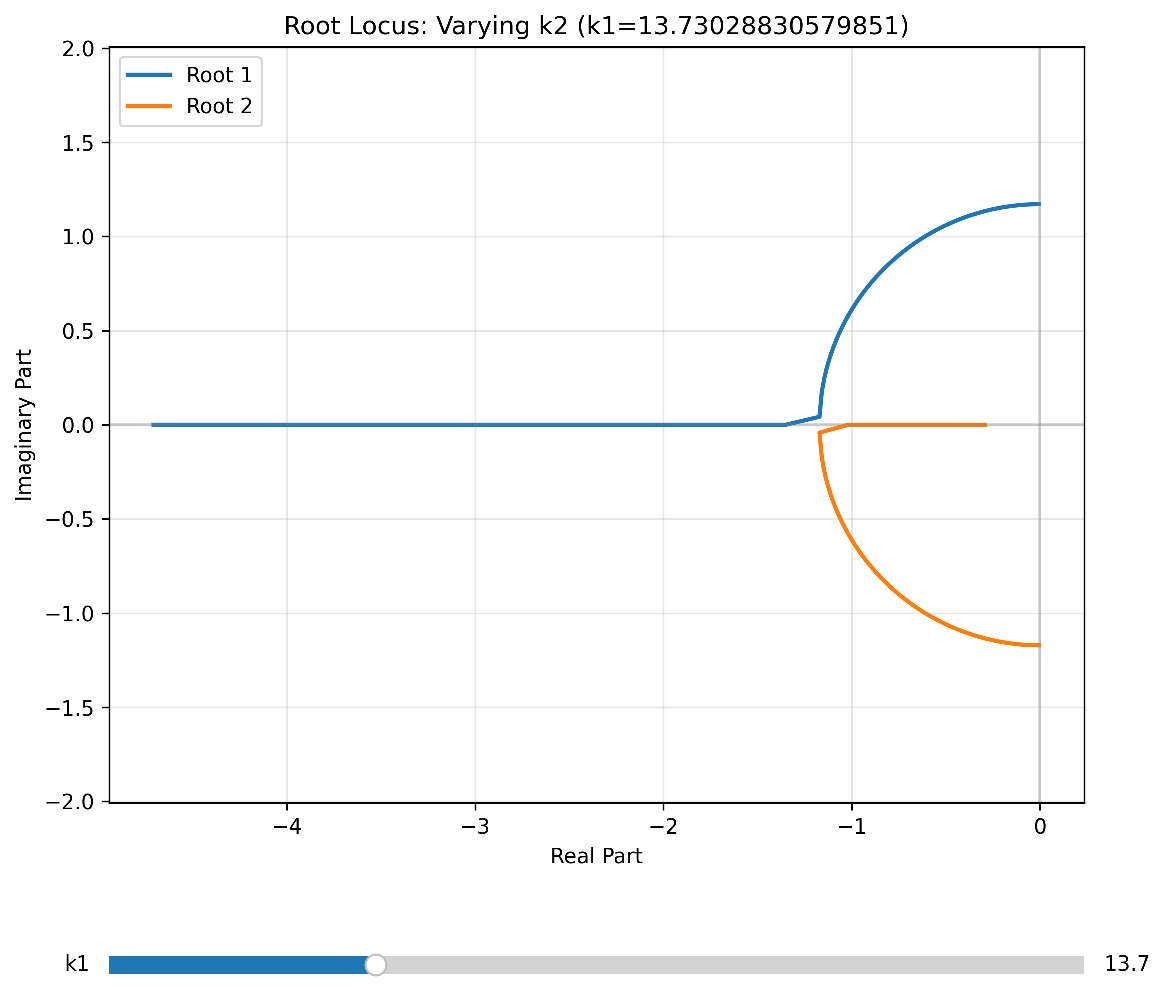
\includegraphics[width=\linewidth]{best_k2_root_locus(4).pdf}
        \caption{Optimized gains}
        \label{fig:subfig2}
    \end{subfigure}
    \caption{Root locus plots for a varying $k_2$ of small spacecraft case 1}
    \label{fig:combined}
\end{figure}
\end{frame}




\section{Conclusion}

% --- Summary ---
\begin{frame}{Summary of Findings}
\begin{itemize}
  \item Optimized PD gains significantly improve performance
  \item Settling time improved by 42\%, torque reduced by $10\times$
  \item Simulation validated across small and large spacecraft
\end{itemize}
\end{frame}

% --- Future Work ---
\begin{frame}{Future Work}
\begin{itemize}
  \item Implement nonlinear controllers (e.g. LQR)
  \item Extend to 3-axis attitude control
  \item Use intelligent gain tuning (e.g. Bayesian optimization)
\end{itemize}
\end{frame}

% --- End ---
\begin{frame}
  \centering
  \Huge\textbf{Thank You!} \\
  \vspace{0.5cm}
  \Large Any Questions?
\end{frame}

\end{document}
